\addtocontents{toc}{\protect\setcounter{tocdepth}{0}}

%\section[]{Appendix}

\begin{frame}
    \frametitle[Classification by Bélády]{Page Replacement Algorithm Classification by Bélády From \cite{Belady:1966}}
    
    \begin{description}
        \item<2-7>[Class 1]    \alt<2-2>{No statistics}{RANDOM, FIFO and FILO}
        \item<4-7>[Class 2]    \alt<4-4>{Statistics about the latest references of \emph{pages in the buffer pool\vspace{\baselineskip}}}{LRU, MRU, LRU-K, SLRU, CLOCK, ZCLOCK, GCLOCK, DGCLOCK, LRD, LFU, LFU-Aging, LFUDA, 2Q, MQ and LeanStore}
        \item<6-7>[Class 3]    \alt<6-6>{Statistics about each time \emph{any page} was fetched from the database and each time it was evicted from the buffer pool}{ARC, CAR, CART, LIRS, CLOCK-Pro, DLIRS and CLOCK-Pro+\vspace{\baselineskip}}
    \end{description}
\end{frame}

%\subsection[]{RANDOM}

%\frame{\subsectionpage}

%\subsection[]{FIFO}

%\frame{\subsectionpage}

%\subsubsection[]{LOOP}

%\frame{\subsubsectionpage}

\begin{frame}
    \frametitle{LOOP Algorithm}

    \centering
    \begin{tikzpicture}[>=latex,
                        semithick,
                        scale = 2.5]
        % Draw the buffer frames in the circular buffer:
        \draw [thick, fill = black!10] (0,0) circle (1);
        \foreach \angle in {90, 67.5, ..., -67.5}
            \draw (\angle:1) -- (\angle-180:1);
        \node [circle, thick, fill = white, draw = black, minimum size = 3.75cm] at (0,0) {\Large \shortstack[c]{Buffer\\pool}};
        
        % Draw the buffer indices:
        \foreach \index/\pageindex in {0/31, 1/52, 2/28, 3/50, 4/11, 5/47, 6/49, 7/23, 8/2, 9/38, 10/43, 11/51, 12/48, 13/56, 14/6, 15/58} {
            \node [visible on = <1>] at (90-11.25-\index*22.5:1.1) {\index};
            \node [visible on = <1>] at (90-11.25-\index*22.5:0.875) {$P_{\pageindex}$};
        }

        % Draw the buffer indices:
        \foreach \index/\pageindex in {0/31, 1/52, 2/28, 3/50, 4/11, 5/47, 6/49, 7/23, 8/2, 9/38, 10/43, 11/51, 12/48, 13/56, 14/6, 15/12} {
            \node [visible on = <2>] at (90-11.25-\index*22.5:1.1) {\index};
            \node [visible on = <2>] at (90-11.25-\index*22.5:0.875) {$P_{\pageindex}$};
        }

        % Draw the buffer indices:
        \foreach \index/\pageindex in {0/19, 1/52, 2/28, 3/50, 4/11, 5/47, 6/49, 7/23, 8/2, 9/38, 10/43, 11/51, 12/48, 13/56, 14/6, 15/12} {
            \node [visible on = <3>] at (90-11.25-\index*22.5:1.1) {\index};
            \node [visible on = <3>] at (90-11.25-\index*22.5:0.875) {$P_{\pageindex}$};
        }

        % Draw the buffer indices:
        \foreach \index/\pageindex in {0/19, 1/52, 2/28, 3/50, 4/11, 5/47, 6/49, 7/23, 8/2, 9/38, 10/43, 11/51, 12/48, 13/56, 14/6, 15/12} {
            \node [visible on = <4>] at (90-11.25-\index*22.5:1.1) {\index};
            \node [visible on = <4>] at (90-11.25-\index*22.5:0.875) {$P_{\pageindex}$};
        }

        % Draw the buffer indices:
        \foreach \index/\pageindex in {0/19, 1/52, 2/28, 3/50, 4/11, 5/47, 6/49, 7/23, 8/2, 9/38, 10/43, 11/51, 12/48, 13/56, 14/6, 15/12} {
            \node [visible on = <5>] at (90-11.25-\index*22.5:1.1) {\index};
            \node [visible on = <5>] at (90-11.25-\index*22.5:0.875) {$P_{\pageindex}$};
        }

        % Draw the buffer indices:
        \foreach \index/\pageindex in {0/19, 1/52, 2/28, 3/50, 4/11, 5/47, 6/49, 7/23, 8/2, 9/38, 10/43, 11/51, 12/48, 13/56, 14/6, 15/12} {
            \node [visible on = <6>] at (90-11.25-\index*22.5:1.1) {\index};
            \node [visible on = <6>] at (90-11.25-\index*22.5:0.875) {$P_{\pageindex}$};
        }

        % Draw the buffer indices:
        \foreach \index/\pageindex in {0/19, 1/52, 2/28, 3/50, 4/30, 5/47, 6/49, 7/23, 8/2, 9/38, 10/43, 11/51, 12/48, 13/56, 14/6, 15/12} {
            \node [visible on = <7>] at (90-11.25-\index*22.5:1.1) {\index};
            \node [visible on = <7>] at (90-11.25-\index*22.5:0.875) {$P_{\pageindex}$};
        }

        % Draw the buffer indices:
        \foreach \index/\pageindex in {0/19, 1/52, 2/28, 3/50, 4/30, 5/47, 6/49, 7/23, 8/2, 9/38, 10/43, 11/51, 12/48, 13/56, 14/6, 15/12} {
            \node [visible on = <8>] at (90-11.25-\index*22.5:1.1) {\index};
            \node [visible on = <8>] at (90-11.25-\index*22.5:0.875) {$P_{\pageindex}$};
        }

        % Draw the buffer indices:
        \foreach \index/\pageindex in {0/19, 1/52, 2/28, 3/50, 4/30, 5/47, 6/49, 7/23, 8/2, 9/38, 10/43, 11/51, 12/48, 13/56, 14/6, 15/12} {
            \node [visible on = <9>] at (90-11.25-\index*22.5:1.1) {\index};
            \node [visible on = <9>] at (90-11.25-\index*22.5:0.875) {$P_{\pageindex}$};
        }

        % Draw the buffer indices:
        \foreach \index/\pageindex in {0/19, 1/52, 2/28, 3/50, 4/30, 5/47, 6/49, 7/58, 8/2, 9/38, 10/43, 11/51, 12/48, 13/56, 14/6, 15/12} {
            \node [visible on = <10>] at (90-11.25-\index*22.5:1.1) {\index};
            \node [visible on = <10>] at (90-11.25-\index*22.5:0.875) {$P_{\pageindex}$};
        }

        % Draw the buffer indices:
        \foreach \index/\pageindex in {0/19, 1/52, 2/28, 3/50, 4/30, 5/47, 6/49, 7/58, 8/27, 9/38, 10/43, 11/51, 12/48, 13/56, 14/6, 15/12} {
            \node [visible on = <11>] at (90-11.25-\index*22.5:1.1) {\index};
            \node [visible on = <11>] at (90-11.25-\index*22.5:0.875) {$P_{\pageindex}$};
        }

        % Draw the buffer indices:
        \foreach \index/\pageindex in {0/19, 1/52, 2/28, 3/50, 4/30, 5/47, 6/49, 7/58, 8/27, 9/38, 10/43, 11/51, 12/48, 13/56, 14/6, 15/12} {
            \node [visible on = <12>] at (90-11.25-\index*22.5:1.1) {\index};
            \node [visible on = <12>] at (90-11.25-\index*22.5:0.875) {$P_{\pageindex}$};
        }

        % Draw the buffer indices:
        \foreach \index/\pageindex in {0/19, 1/52, 2/28, 3/50, 4/30, 5/47, 6/49, 7/58, 8/27, 9/38, 10/43, 11/51, 12/48, 13/56, 14/6, 15/12} {
            \node [visible on = <13>] at (90-11.25-\index*22.5:1.1) {\index};
            \node [visible on = <13>] at (90-11.25-\index*22.5:0.875) {$P_{\pageindex}$};
        }

        % Draw the buffer indices:
        \foreach \index/\pageindex in {0/19, 1/52, 2/28, 3/50, 4/30, 5/47, 6/49, 7/58, 8/27, 9/38, 10/43, 11/51, 12/48, 13/56, 14/6, 15/12} {
            \node [visible on = <14>] at (90-11.25-\index*22.5:1.1) {\index};
            \node [visible on = <14>] at (90-11.25-\index*22.5:0.875) {$P_{\pageindex}$};
        }

        % Draw the buffer indices:
        \foreach \index/\pageindex in {0/19, 1/52, 2/28, 3/50, 4/30, 5/47, 6/49, 7/58, 8/27, 9/38, 10/43, 11/51, 12/48, 13/56, 14/6, 15/12} {
            \node [visible on = <15>] at (90-11.25-\index*22.5:1.1) {\index};
            \node [visible on = <15>] at (90-11.25-\index*22.5:0.875) {$P_{\pageindex}$};
        }

        % Draw the buffer indices:
        \foreach \index/\pageindex in {0/19, 1/52, 2/28, 3/50, 4/30, 5/47, 6/49, 7/58, 8/27, 9/38, 10/43, 11/51, 12/48, 13/34, 14/6, 15/12} {
            \node [visible on = <16>] at (90-11.25-\index*22.5:1.1) {\index};
            \node [visible on = <16>] at (90-11.25-\index*22.5:0.875) {$P_{\pageindex}$};
        }

        % Draw the buffer indices:
        \foreach \index/\pageindex in {0/19, 1/52, 2/28, 3/50, 4/30, 5/47, 6/49, 7/58, 8/27, 9/38, 10/43, 11/51, 12/48, 13/34, 14/13, 15/12} {
            \node [visible on = <17>] at (90-11.25-\index*22.5:1.1) {\index};
            \node [visible on = <17>] at (90-11.25-\index*22.5:0.875) {$P_{\pageindex}$};
        }

        \foreach \frame/\index in {1/14\ignore{, 2/15, 3/0, 4/1, 5/2, 6/3, 7/4, 8/5, 9/6, 10/7, 11/8, 12/9, 13/10, 14/11, 15/12, 16/13, 17/14}} {   
            \ifthenelse{\index = 0 \OR \index = 1 \OR \index = 2 \OR \index = 3 \OR \index = 4 \OR \index = 5 \OR \index = 6 \OR \index = 7}{     
                \draw [<-, visible on = <\frame>] (90-11.25-\index*22.5:1.2) -- (90-11.25-\index*22.5:1.333) -- +(.125,0) node [left, inner xsep = .125cm, anchor = west, visible on = <\frame>] (Tail) {Tail};
            }{
                \draw [<-, visible on = <\frame>] (90-11.25-\index*22.5:1.2) -- (90-11.25-\index*22.5:1.333) -- +(-.125,0) node [right, inner xsep = .125cm, anchor = east, visible on = <\frame>] (Tail) {Tail};
            }
        }
        \foreach \frame/\index in {1/15\ignore{, 2/0, 3/1, 4/2, 5/3, 6/4, 7/5, 8/6, 9/7, 10/8, 11/9, 12/10, 13/11, 14/12, 15/13, 16/14, 17/15}} {   
            \ifthenelse{\index = 0 \OR \index = 1 \OR \index = 2 \OR \index = 3 \OR \index = 4 \OR \index = 5 \OR \index = 6 \OR \index = 7}{     
                \draw [<-, visible on = <\frame>] (90-11.25-\index*22.5:1.2) -- (90-11.25-\index*22.5:1.333) -- +(.125,0) node [left, inner xsep = .125cm, anchor = west, visible on = <\frame>] (Head) {Head};
            }{
                \draw [<-, visible on = <\frame>] (90-11.25-\index*22.5:1.2) -- (90-11.25-\index*22.5:1.333) -- +(-.125,0) node [right, inner xsep = .125cm, anchor = east, visible on = <\frame>] (Head) {Head};
            }
        }
        \draw [->, thick, visible on = <1>] (0,0)+(90:1.333) arc [start angle = 90, end angle = 45, radius = 1.333];
    \end{tikzpicture}
\end{frame}

%\subsubsection[]{Quasi-FIFO}

%\frame{\subsubsectionpage}

\begin{frame}
    \frametitle{Quasi-FIFO Algorithm}

    \tikzset{%
        every picture/.append style = {>=latex,
                                       thick,
                                       scale = 2.375}
    }

    \centering
    \vspace{-2em}
    \begin{minipage}{.6\columnwidth}
        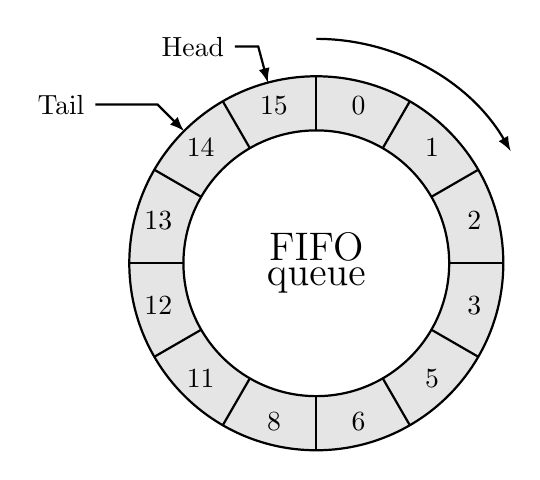
\begin{tikzpicture}
            % Draw the FIFO queue:
            \draw [fill = black!10] (0,0) circle (1);
            \foreach \angle in {90, 60, ..., -60}
                \draw (\angle:1) -- (\angle-180:1);
            \node [circle, fill = white, draw = black, minimum size = 3.375cm] at (0,0) {\Large \shortstack[c]{FIFO\\queue}};
            
            % Draw the buffer indices:
            \node [] at ( 75:0.875)  {0};
            \node [] at  (45:0.875)  {1};
            \node [] at ( 15:0.875)  {2};
            \node [] at (345:0.875)  {3};
            \node [] at (315:0.875)  {5};
            \node [] at (285:0.875)  {6};
            \node [] at (255:0.875)  {8};
            \node [] at (225:0.875) {11};
            \node [] at (195:0.875) {12};
            \node [] at (165:0.875) {13};
            \node [] at (135:0.875) {14};
            \node [] at (105:0.875) {15};
            
            \draw [<-] (135:1) -- (135:1.2) -- +(-.333,0)
                node [right, inner xsep = .125cm, anchor = east] (Tail) {Tail};
            \draw [<-] (105:1) -- (105:1.2) -- +(-.125,0)
                node [right, inner xsep = .125cm, anchor = east] (Head) {Head};
            \draw [->] (0,0)+(90:1.2) arc [start angle = 90, end angle = 30, radius = 1.2];
        \end{tikzpicture}%
    \end{minipage}%
    \begin{minipage}{.4\columnwidth}
        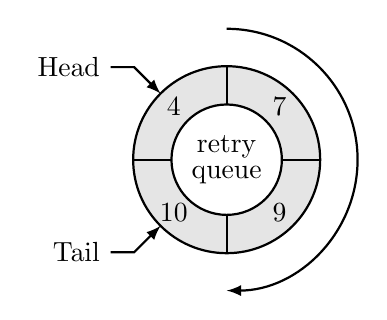
\begin{tikzpicture}
            % Draw the retry queue:
            \draw [fill = black!10] (0,0) circle (.5);
            \foreach \angle in {90, 0}
                \draw (\angle:.5) -- (\angle-180:.5);
            \node [circle, fill = white, draw = black, minimum size = 1.125cm] at (0,0) {\shortstack[c]{retry\\queue}};
            
            % Draw the buffer indices:
            \node [] at ( 45:0.4)  {7};
            \node [] at (315:0.4)  {9};
            \node [] at (225:0.4) {10};
            \node [] at (135:0.4)  {4};
            
            \draw [<-] (225:.5) -- (225:.7) -- +(-.125,0)
                node [right, inner xsep = .125cm, anchor = east] (Tail) {Tail};
            \draw [<-] (135:.5) -- (135:.7) -- +(-.125,0)
                node [right, inner xsep = .125cm, anchor = east] (Head) {Head};
            \draw [->, thick] (0,0)+(90:.7) arc [start angle = 90, end angle = -90, radius = .7];
        \end{tikzpicture}
    \end{minipage} \\
    \vspace{-.5em}
    \begin{tikzpicture}[boolRectangle/.style = {draw = black,
                                                thick,
                                                rectangle}]
        \node [draw = none]  (currentlyCheckingRetryQueue)               {currentlyCheckingRetryQueue};
        \node [boolRectangle, right = 0em of currentlyCheckingRetryQueue, fill = black!10] (currentlyCheckingRetryQueueValue) {true};
        \node [draw = none, right = 3em of currentlyCheckingRetryQueue] (currentQueueChecks) {currentQueueChecks};
        \node [rectangle, draw = black, right = 0em of currentQueueChecks, fill = black!10] (currentQueueChecksValue) {15};
        \node[rectangle, draw = black, inner sep = .15em, fit = (currentlyCheckingRetryQueue)(currentlyCheckingRetryQueueValue)(currentQueueChecks)(currentQueueChecksValue), label = {Thread 0}] {};
    \end{tikzpicture} \\
    \vspace{-.125em}
    \begin{tikzpicture}[font = \small,
                        label distance = -2.5pt,
                        boolRectangle/.style = {draw = black,
                                                thick,
                                                rectangle,
                                                inner xsep = .1111em,
                                                fill = black!10}]
        \node [boolRectangle, label = below: 0]                             (index0) {true};
        \node [boolRectangle, label = below: 1, right = -0.8pt of  index0]  (index1) {true};
        \node [boolRectangle, label = below: 2, right = -0.8pt of  index1]  (index2) {true};
        \node [boolRectangle, label = below: 3, right = -0.8pt of  index2]  (index3) {true};
        \node [boolRectangle, label = below: 4, right = -0.8pt of  index3]  (index4) {true};
        \node [boolRectangle, label = below: 5, right = -0.8pt of  index4]  (index5) {true};
        \node [boolRectangle, label = below: 6, right = -0.8pt of  index5]  (index6) {true};
        \node [boolRectangle, label = below: 7, right = -0.8pt of  index6]  (index7) {true};
        \node [boolRectangle, label = below: 8, right = -0.8pt of  index7]  (index8) {true};
        \node [boolRectangle, label = below: 9, right = -0.8pt of  index8]  (index9) {true};
        \node [boolRectangle, label = below:10, right = -0.8pt of  index9] (index10) {true};
        \node [boolRectangle, label = below:11, right = -0.8pt of index10] (index11) {true};
        \node [boolRectangle, label = below:12, right = -0.8pt of index11] (index12) {true};
        \node [boolRectangle, label = below:13, right = -0.8pt of index12] (index13) {true};
        \node [boolRectangle, label = below:14, right = -0.8pt of index13] (index14) {true};
        \node [boolRectangle, label = below:15, right = -0.8pt of index14] (index15) {true};
        
        \node [above = 1.25em of index0.west, anchor = west]{notExplicitlyEvictedList};
    \end{tikzpicture}
\end{frame}

%\subsection[]{FILO}

%\frame{\subsectionpage}

%\subsection[]{Most Recently Used}

%\frame{\subsectionpage}

%\subsubsection[]{Quasi-MRU}

%\frame{\subsubsectionpage}

%\subsection[]{LRU-K \cite{ONeil:1993}}

%\frame{\subsectionpage}

\begin{frame}
    \frametitle{LRU-K Implementations}

    \begin{itemize}
        \item<2->   \emph{Hash-Map-Doubly-Linked-List}
                    \begin{itemize}
                        \item<3->   Entries in the queue are reference IDs instead of frame indexes
                        \item<4->   Ghost references\uncover<5->{\footnote<5->[frame]{Ghost references are used for pages with $<k$ references}} are in a segment at the head of the queue
                    \end{itemize}
        \item<6->   \emph{Timestamp-Sorting}
                    \begin{itemize}
                        \item<7->   $k$ timestamps per buffer frame
                        \item<8->   Ghost references are represented by timestamps very early in the past
                    \end{itemize}
    \end{itemize}
\end{frame}

%\subsubsection[]{Hash-Map-Doubly-Linked-List Implementation}

%\frame{\subsubsectionpage}

%\subsubsection[]{Timestamp-Sorting Implementation}

%\frame{\subsubsectionpage}

%\subsection[]{Segmented LRU \cite{Karedla:1994}}

%\frame{\subsectionpage}

%\subsection[]{CLOCK \cite{Corbato:1969}}

%\frame{\subsectionpage}

\begin{frame}
    \frametitle{CLOCK Variants}

    \tikzset{%
        node distance = 1cm,
        refBit/.style = {draw = black, shape = rectangle, rounded corners = 1pt, fill = black!10},
        hand/.style = {very thick, draw = black}
    }

    \centering
    \begin{minipage}{.65\textwidth}
        \begin{description}
            \item<2->[Fix] Set usage-bit on \emph{page fix}
            \item<3->[Unfix] Set usage-bit on \emph{page unfix}
            \item<4->[FixUnfix] Set usage-bit on \emph{page fix} and on \emph{page unfix}
            \item<5->[Full] Like \textcolor{structure}{FixUnfix} but also set usage-bit when page cannot be evicted
        \end{description}
    \end{minipage}
    \begin{minipage}{.325\textwidth}
        \resizebox{\linewidth}{!}{
            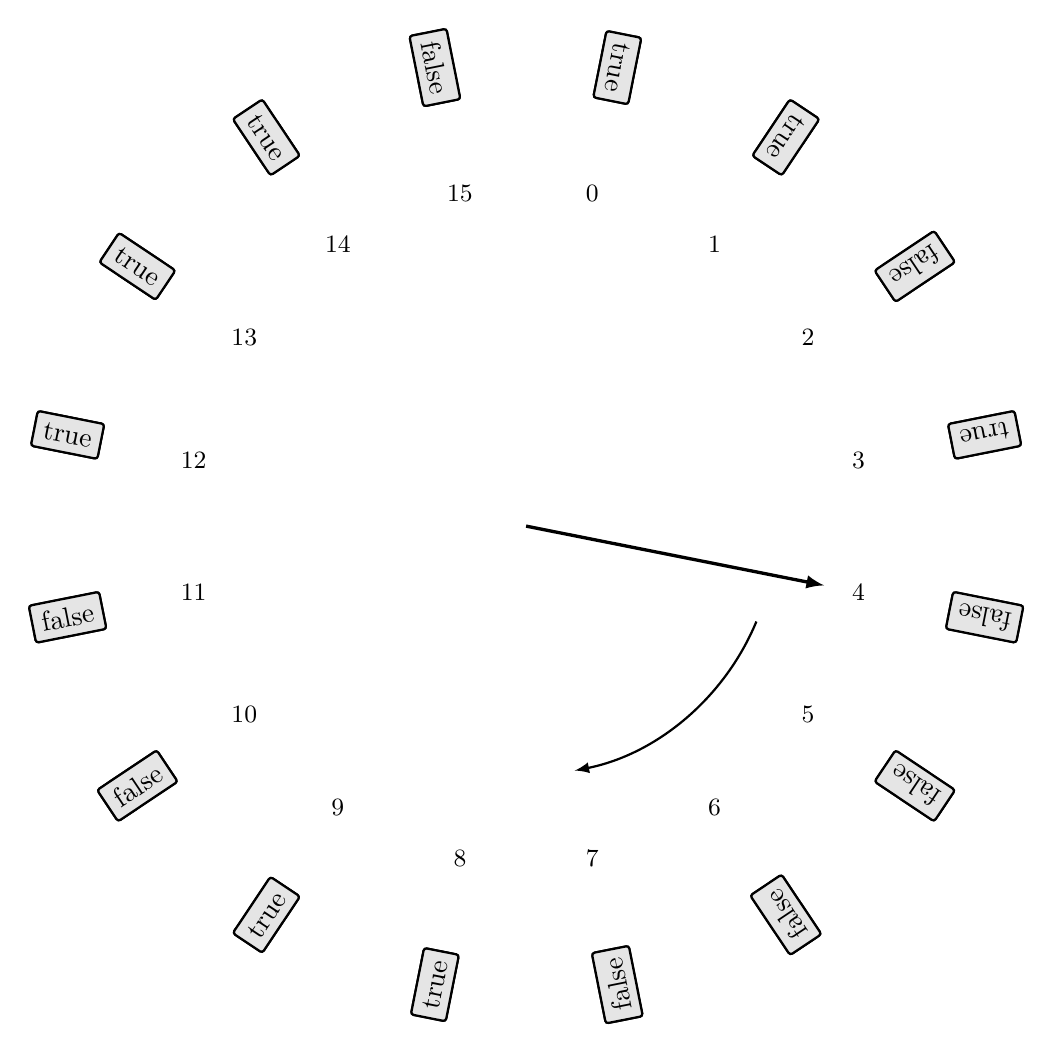
\begin{tikzpicture}
                \foreach \index/\referenced in {0/true, 1/true, 2/false, 3/true, 4/false, 5/false, 6/false, 7/false, 8/true, 9/true, 10/false, 11/false, 12/true, 13/true, 14/true, 15/false} {
                    \ifthenelse{\index < 8}{%
                        \node [refBit, rotate = 90-11.25-\index*22.5] at (90-11.25-\index*22.5:2.5) {\referenced};%
                    }{%
                        \node [refBit, rotate = 270-11.25-\index*22.5] at (90-11.25-\index*22.5:2.5) {\referenced};%
                    }
                    \node [draw = none, font = \small] at (90-11.25-\index*22.5:1.8125) {\index};
                }
                \path[->] (0,0)		edge[hand]		(-11.25:1.625);
                \draw [->, thick] (0,0)+(-22.5:1.333) arc [start angle = -22.5, end angle = -78.75, radius = 1.333];
            \end{tikzpicture}
        }
    \end{minipage}
\end{frame}

\begin{frame}
    \frametitle{Performance Evaluation}

    \pgfplotsset{%
        every axis/.append style = {
            yticklabel style = {font = \scriptsize},
            scaled y ticks = false,
            ybar = .8pt,
            bar width = .5em,
            xmin = -0.75,
            xmax = 7.75,
            xtick style = {draw = none},
            xtick = {0, 1, 2, 3, 4, 5, 6, 7},
            xticklabels = {{\SI{0.1}{\giga\byte}}, {\SI{0.5}{\giga\byte}}, {\SI{1}{\giga\byte}}, {\SI{2.5}{\giga\byte}}, {\SI{5}{\giga\byte}}, {\SI{10}{\giga\byte}}, {\SI{20}{\giga\byte}}, {\SI{30}{\giga\byte}}},
            x tick label style = {align = center,
                                  font = \footnotesize},
            width = .925\textwidth,
            height = .8\paperheight
        }
    }

    \tikzset{%
        fix/.style = {thick, draw = Cerulean, fill = Cerulean!50},
        unfix/.style = {thick, draw = Magenta, fill = Magenta!50},
        fixunfix/.style = {thick, draw = blue, fill = blue!50},
        full/.style = {thick, draw = black, fill = black!50},
        missrate/.style = {mark = *}
    }

    \begin{tikzpicture}
        \begin{axis}[ymode = normal,
                     ymin = 0,
                     ymax = 1000000,
                     ymajorgrids = true,
                     yticklabel style = {/pgf/number format/fixed},
                     legend entries = {Fix, Unfix, FixUnfix, \alert<3->{Full}},
                     legend style = {font = \tiny,
                                     legend columns = -1,
                                     /tikz/every even column/.append style = {column sep = 0.05cm},
                                     row sep = -2pt,
                                     draw = none,
                                     fill = none,
                                     at = {(0.5, 0.97)},
                                     anchor = north}]
            \addplot[fix, visible on = <2->] coordinates
                {(0, 64101.70) (1, 79671.85) (2, 92642.61) (3, 142191.06) (4, 248060.53) (5, 618312.54) (6, 765080.14) (7, 884937.94)};
            \addplot[unfix, visible on = <2->] coordinates
                {(0, 65258.34) (1, 80603.40) (2, 91767.14) (3, 142441.22) (4, 243736.23) (5, 626089.00) (6, 755520.72) (7, 883699.37)};
            \addplot[fixunfix, visible on = <2->] coordinates
                {(0, 65841.74) (1, 79656.75) (2, 94042.93) (3, 143951.26) (4, 244904.41) (5, 623828.48) (6, 771109.94) (7, 887411.97)};
            \addplot[full, visible on = <2->] coordinates
                {(0, 66889.87) (1, 79510.40) (2, 96140.14) (3, 143675.28) (4, 253828.17) (5, 644553.46) (6, 765998.78) (7, 887183.25)};
        \end{axis}
        \begin{axis}[axis y line* = right,
                     ymode = normal,
                     ymin = 100,
                     ymax = 75,
                     grid = none,
                     ycomb = .8pt,
                     y coord trafo/.code = {
                         \pgfmathparse{100 - ####1}
                         \pgfmathresult
                     },
                     yticklabel={\SI[round-mode = places, round-precision = 0]{\tick}{\percent}}]
            \addplot[fix, missrate, xshift = -9.5, visible on = <3->] coordinates
                {(0, 79.49) (1, 88.81) (2, 92.38) (3, 96.46) (4, 98.28) (5, 99.71) (6, 99.85) (7, 99.86)};
            \addplot[unfix, missrate, xshift = -3.167, visible on = <3->] coordinates
                {(0, 79.48) (1, 88.83) (2, 92.39) (3, 96.48) (4, 98.27) (5, 99.71) (6, 99.85) (7, 99.86)};
            \addplot[fixunfix, missrate, xshift = 3.167, visible on = <3->] coordinates
                {(0, 79.49) (1, 88.84) (2, 92.40) (3, 96.46) (4, 98.26) (5, 99.71) (6, 99.85) (7, 99.86)};
            \addplot[full, missrate, xshift = 9.5, visible on = <3->] coordinates
                {(0, 78.22) (1, 87.52) (2, 92.12) (3, 96.29) (4, 98.25) (5, 99.65) (6, 99.85) (7, 99.86)};
        \end{axis}
    \end{tikzpicture}
\end{frame}

%\subsection[]{Zero-Handed CLOCK}

%\frame{\subsectionpage}

\begin{frame}
    \frametitle{ZCLOCK Variants}

    \begin{description}
        \item[Fix] Set usage-bit on \emph{page fix}
        \item[Unfix] Set usage-bit on \emph{page unfix}
        \item[FixUnfix] Set usage-bit on \emph{page fix} and on \emph{page unfix}
        \item[Full] Like \textcolor{structure}{FixUnfix} but also set usage-bit when page cannot be evicted
    \end{description}
\end{frame}

\begin{frame}
    \frametitle{Performance Evaluation}

    \pgfplotsset{%
        every axis/.append style = {
            yticklabel style = {font = \scriptsize},
            scaled y ticks = false,
            ybar = .8pt,
            bar width = .5em,
            xmin = -0.75,
            xmax = 7.75,
            xtick style = {draw = none},
            xtick = {0, 1, 2, 3, 4, 5, 6, 7},
            xticklabels = {{\SI{0.1}{\giga\byte}}, {\SI{0.5}{\giga\byte}}, {\SI{1}{\giga\byte}}, {\SI{2.5}{\giga\byte}}, {\SI{5}{\giga\byte}}, {\SI{10}{\giga\byte}}, {\SI{20}{\giga\byte}}, {\SI{30}{\giga\byte}}},
            x tick label style = {align = center,
                                  font = \footnotesize},
            width = .925\textwidth,
            height = .8\paperheight
        }
    }

    \tikzset{%
        fix/.style = {thick, draw = Cerulean, fill = Cerulean!50},
        unfix/.style = {thick, draw = Magenta, fill = Magenta!50},
        fixunfix/.style = {thick, draw = blue, fill = blue!50},
        full/.style = {thick, draw = black, fill = black!50},
        missrate/.style = {mark = *}
    }

    \begin{tikzpicture}
        \begin{axis}[ymode = normal,
                     ymin = 0,
                     ymax = 1000000,
                     ymajorgrids = true,
                     yticklabel style = {/pgf/number format/fixed},
                     legend entries = {\alert<3->{Fix}, Unfix, FixUnfix, Full},
                     legend style = {font = \tiny,
                                     legend columns = -1,
                                     /tikz/every even column/.append style = {column sep = 0.05cm},
                                     row sep = -2pt,
                                     draw = none,
                                     fill = none,
                                     at = {(0.5, 0.97)},
                                     anchor = north}]
            \addplot[fix] coordinates
                {(0, 68497.96) (1, 81310.75) (2, 95666.51) (3, 141048.76) (4, 257937.87) (5, 748964.14) (6, 831333.07) (7, 887381.33)};
            \addplot[unfix] coordinates
                {(0, 68735.66) (1, 81235.53) (2, 95112.94) (3, 141372.05) (4, 252519.35) (5, 740675.06) (6, 826589.22) (7, 887066.52)};
            \addplot[fixunfix] coordinates
                {(0, 66262.42) (1, 79199.88) (2, 94841.88) (3, 140062.95) (4, 250143.61) (5, 732804.97) (6, 820238.34) (7, 884463.27)};
            \addplot[full] coordinates
                {(0, 67929.24) (1, 79571.06) (2, 96412.80) (3, 141834.10) (4, 254240.30) (5, 639458.83) (6, 752035.27) (7, 887811.83)};
        \end{axis}
        \begin{axis}[axis y line* = right,
                     ymode = normal,
                     ymin = 100,
                     ymax = 75,
                     grid = none,
                     ycomb = .8pt,
                     y coord trafo/.code = {
                         \pgfmathparse{100 - ####1}
                         \pgfmathresult
                     },
                     yticklabel={\SI[round-mode = places, round-precision = 0]{\tick}{\percent}}]
            \addplot[fix, missrate, xshift = -9.5, visible on = <2->] coordinates
                {(0, 78.52) (1, 87.23) (2, 91.73) (3, 96.26) (4, 98.29) (5, 99.65) (6, 99.85) (7, 99.86)};
            \addplot[unfix, missrate, xshift = -3.167, visible on = <2->] coordinates
                {(0, 79.13) (1, 87.38) (2, 91.73) (3, 96.27) (4, 98.28) (5, 99.66) (6, 99.85) (7, 99.86)};
            \addplot[fixunfix, missrate, xshift = 3.167, visible on = <2->] coordinates
                {(0, 79.13) (1, 87.42) (2, 91.74) (3, 96.28) (4, 98.26) (5, 99.66) (6, 99.85) (7, 99.86)};
            \addplot[full, missrate, xshift = 9.5, visible on = <2->] coordinates
                {(0, 78.23) (1, 87.51) (2, 92.12) (3, 96.31) (4, 98.25) (5, 99.65) (6, 99.85) (7, 99.86)};
        \end{axis}
    \end{tikzpicture}
\end{frame}

%\subsection[]{Generalized CLOCK \cite{Effelsberg:1984}}

%\frame{\subsectionpage}

%\subsubsection[]{GCLOCK-V1}

%\frame{\subsubsectionpage}

\begin{frame}
    \frametitle{GCLOCK-V1 Variants}

    \tikzset{%
        node distance = 1cm,
        refInt/.style = {draw = black, shape = rectangle, rounded corners = 1pt, fill = black!10},
        hand/.style = {very thick, draw = black}
    }

    \begin{block}{Usage-Count}
        \vspace{-2em}
        \begin{align*}
            \text{(initially)\qquad}\text{UC}\left(p\right) &= F\\
            \text{(increase)\qquad}\text{UC}\left(p\right) &= \text{UC}\left(p\right) + R\\
            \text{(decrease)\qquad}\text{UC}\left(p\right) &= \text{UC}\left(p\right) - 1
        \end{align*}
        \vspace{-1.5em}
    \end{block}

    \centering
    \begin{minipage}{.65\textwidth}
        \footnotesize
        \begin{description}
            \item<2->[Fix]          Increase usage-count on \emph{page fix}
            \item<3->[FixFull]      Like \textcolor{structure}{Fix} but also increase usage-count when page cannot be evicted
            \item<4->[Unfix]        Increase usage-count on \emph{page unfix}
            \item<5->[UnfixFull]    Like \textcolor{structure}{Unfix} but also increase usage-count when page cannot be evicted
        \end{description}
        \vspace{.5em}
        \begin{description}
            \item<6->[]     $F = 25$, $R = 5$
            \item<7->[x2]   $F = 50$, $R = 10$
        \end{description}
    \end{minipage}
    \begin{minipage}{.3\textwidth}
        \resizebox{\linewidth}{!}{
            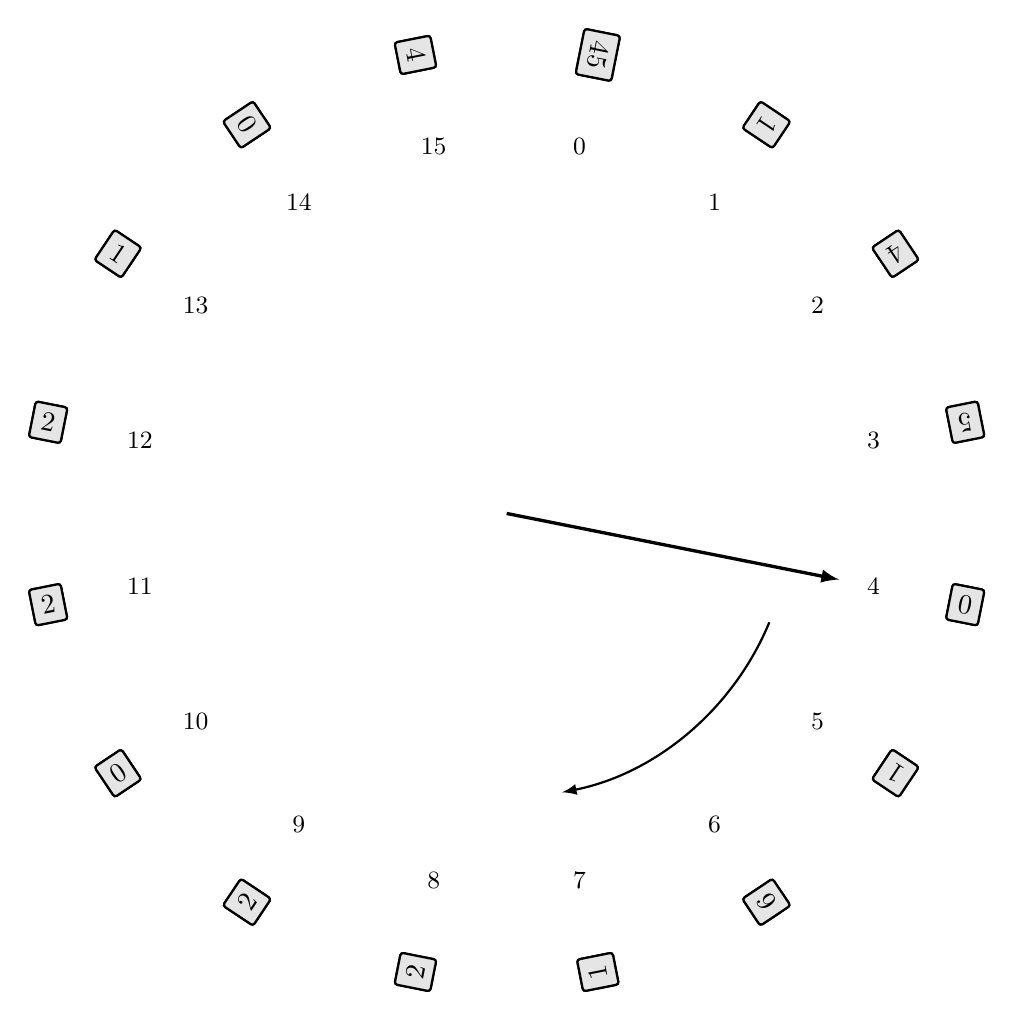
\begin{tikzpicture}
                \foreach \index/\referenced in {0/45, 1/1, 2/4, 3/5, 4/0, 5/1, 6/6, 7/1, 8/2, 9/2, 10/0, 11/2, 12/2, 13/1, 14/0, 15/4} {
                    \ifthenelse{\index < 8}{%
                        \node [refInt, rotate = 90-11.25-\index*22.5] at (90-11.25-\index*22.5:2.5) {\referenced};%
                    }{%
                        \node [refInt, rotate = 270-11.25-\index*22.5] at (90-11.25-\index*22.5:2.5) {\referenced};%
                    }
                    \node [draw = none, font = \small] at (90-11.25-\index*22.5:2) {\index};
                }
                \path[->] (0,0)		edge[hand]		(-11.25:1.8125);
                \draw [->, thick] (0,0)+(-22.5:1.5205) arc [start angle = -22.5, end angle = -78.75, radius = 1.5205];
            \end{tikzpicture}
        }
    \end{minipage}
    
\end{frame}

\begin{frame}
    \frametitle{Performance Evaluation}

    \pgfplotsset{%
        every axis/.append style = {
            yticklabel style = {font = \scriptsize},
            scaled y ticks = false,
            ybar = .8pt,
            bar width = .225em,
            xmin = -0.75,
            xmax = 7.75,
            xtick style = {draw = none},
            xtick = {0, 1, 2, 3, 4, 5, 6, 7},
            xticklabels = {{\SI{0.1}{\giga\byte}}, {\SI{0.5}{\giga\byte}}, {\SI{1}{\giga\byte}}, {\SI{2.5}{\giga\byte}}, {\SI{5}{\giga\byte}}, {\SI{10}{\giga\byte}}, {\SI{20}{\giga\byte}}, {\SI{30}{\giga\byte}}},
            x tick label style = {align = center,
                                  font = \footnotesize},
            width = .925\textwidth,
            height = .8\paperheight
        }
    }

    \tikzset{%
        fix/.style = {thick, draw = Cerulean!50, fill = Cerulean!25},
        fixfull/.style = {thick, draw = Cerulean, fill = Cerulean!50},
        unfix/.style = {thick, draw = Magenta!50, fill = Magenta!25},
        unfixfull/.style = {thick, draw = Magenta, fill = Magenta!50},
        x2/.style = {dashed},
        missrate/.style = {mark = *}
    }

    \begin{tikzpicture}
        \begin{axis}[ymode = normal,
                     ymin = 0,
                     ymax = 1000000,
                     ymajorgrids = true,
                     yticklabel style = {/pgf/number format/fixed},
                     legend style = {font = \tiny,
                                     legend columns = 4,
                                     /tikz/every even column/.append style = {column sep = 0.05cm},
                                     row sep = -2pt,
                                     draw = none,
                                     fill = none,
                                     at = {(0.5, 0.97)},
                                     anchor = north}]
            \addplot[fix] coordinates
                {(0, 65049.45) (1, 78530.77) (2, 88025.23) (3, 125866.02) (4, 187490.74) (5, 404662.39) (6, 675934.32) (7, 881666.37)};
            \addlegendentry{Fix};
            \addplot[fixfull] coordinates
                {(0, 65360.99) (1, 83246.02) (2, 91920.02) (3, 129170.52) (4, 202754.77) (5, 476000.85) (6, 689875.86) (7, 882042.46)};
            \addlegendentry{\alert<4->{FixFull}};
            \addplot[unfix] coordinates
                {(0, 66291.95) (1, 78447.75) (2, 89785.49) (3, 127051.88) (4, 186308.27) (5, 405952.72) (6, 674918.45) (7, 869788.30)};
            \addlegendentry{Unfix};
            \addplot[unfixfull] coordinates
                {(0, 64561.13) (1, 81396.24) (2, 90398.24) (3, 132267.48) (4, 202467.74) (5, 475327.68) (6, 684862.90) (7, 882622.07)};
            \addlegendentry{UnfixFull};
            \addplot[fix, x2, visible on = <2->] coordinates
                {(0, 65053.38) (1, 75641.80) (2, 87839.72) (3, 125580.15) (4, 177340.18) (5, 350625.16) (6, 655014.83) (7, 890546.99)};
            \addlegendentry[visible on = <2->]{Fixx2};
            \addplot[fixfull, x2, visible on = <2->] coordinates
                {(0, 65077.68) (1, 77498.27) (2, 91237.39) (3, 129569.02) (4, 201051.50) (5, 444821.84) (6, 672896.71) (7, 883866.71)};
            \addlegendentry[visible on = <2->]{FixFullx2};
            \addplot[unfix, x2, visible on = <2->] coordinates
                {(0, 63763.35) (1, 76889.43) (2, 87512.01) (3, 124617.60) (4, 176894.46) (5, 354239.62) (6, 653033.24) (7, 879953.96)};
            \addlegendentry[visible on = <2->]{Unfixx2};
            \addplot[unfixfull, x2, visible on = <2->] coordinates
                {(0, 65271.86) (1, 80203.53) (2, 90558.15) (3, 129200.63) (4, 198557.05) (5, 445591.47) (6, 674298.46) (7, 888827.20)};
            \addlegendentry[visible on = <2->]{UnfixFullx2};
        \end{axis}
        \begin{axis}[axis y line* = right,
                     ymode = normal,
                     ymin = 100,
                     ymax = 75,
                     grid = none,
                     ycomb = .8pt,
                     y coord trafo/.code = {
                         \pgfmathparse{100 - ####1}
                         \pgfmathresult
                     },
                     yticklabel={\SI[round-mode = places, round-precision = 0]{\tick}{\percent}}]
                \addplot[fix, missrate, xshift = -11.5, visible on = <3->] coordinates
                    {(0, 81.50) (1, 89.54) (2, 92.00) (3, 95.99) (4, 97.83) (5, 99.45) (6, 99.84) (7, 99.86)};
                \addplot[fixfull, missrate, xshift = -8.21, visible on = <3->] coordinates
                    {(0, 80.38) (1, 89.42) (2, 92.16) (3, 96.09) (4, 97.86) (5, 99.47) (6, 99.84) (7, 99.86)};
                \addplot[unfix, missrate, xshift = -4.93, visible on = <3->] coordinates
                    {(0, 81.64) (1, 89.54) (2, 92.02) (3, 96.02) (4, 97.82) (5, 99.45) (6, 99.84) (7, 99.86)};
                \addplot[unfixfull, missrate, xshift = -1.64, visible on = <3->] coordinates
                    {(0, 80.60) (1, 89.37) (2, 92.16) (3, 96.10) (4, 97.87) (5, 99.47) (6, 99.84) (7, 99.86)};
                \addplot[fix, x2, missrate, xshift = 1.64, visible on = <3->] coordinates
                    {(0, 82.47) (1, 89.48) (2, 91.88) (3, 95.93) (4, 97.82) (5, 99.46) (6, 99.84) (7, 99.86)};
                \addplot[fixfull, x2, missrate, xshift = 4.93, visible on = <3->] coordinates
                    {(0, 80.91) (1, 89.47) (2, 92.07) (3, 96.02) (4, 97.86) (5, 99.46) (6, 99.84) (7, 99.86)};
                \addplot[unfix, x2, missrate, xshift = 8.21, visible on = <3->] coordinates
                    {(0, 82.52) (1, 89.49) (2, 91.89) (3, 95.93) (4, 97.82) (5, 99.46) (6, 99.84) (7, 99.86)};
                \addplot[unfixfull, x2, missrate, xshift = 11.5, visible on = <3->] coordinates
                    {(0, 81.08) (1, 89.46) (2, 92.08) (3, 96.02) (4, 97.85) (5, 99.46) (6, 99.84) (7, 99.86)};
        \end{axis}
    \end{tikzpicture}
\end{frame}

%\subsubsection[]{GCLOCK-V2}

%\frame{\subsubsectionpage}

\begin{frame}
    \frametitle{GCLOCK-V2 Variants}

    \tikzset{%
        node distance = 1cm,
        refInt/.style = {draw = black, shape = rectangle, rounded corners = 1pt, fill = black!10},
        hand/.style = {very thick, draw = black}
    }

    \begin{block}<2->{Usage-Count}
        \vspace{-2em}
        \begin{align*}
            \text{(initially)\qquad}\text{UC}\left(p\right) &= F\\
            \text{(set)\qquad}\text{UC}\left(p\right) &= R\\
            \text{(decrease)\qquad}\text{UC}\left(p\right) &= \text{UC}\left(p\right) - 1
        \end{align*}
        \vspace{-1.5em}
    \end{block}

    \centering
    \begin{minipage}{.65\textwidth}
        \footnotesize
        \begin{description}
            \item[Fix]          Set usage-count on \emph{page fix}
            \item[FixFull]      Like \textcolor{structure}{Fix} but also set usage-count when page cannot be evicted
            \item[Unfix]        Set usage-count on \emph{page unfix}
            \item[UnfixFull]    Like \textcolor{structure}{Unfix} but also set usage-count when page cannot be evicted
        \end{description}
        \vspace{.5em}
        \begin{description}
            \item[]     $F = 25$, $R = 5$
            \item[x2]   $F = 50$, $R = 10$
        \end{description}
    \end{minipage}
    \begin{minipage}{.3\textwidth}
        \resizebox{\linewidth}{!}{
            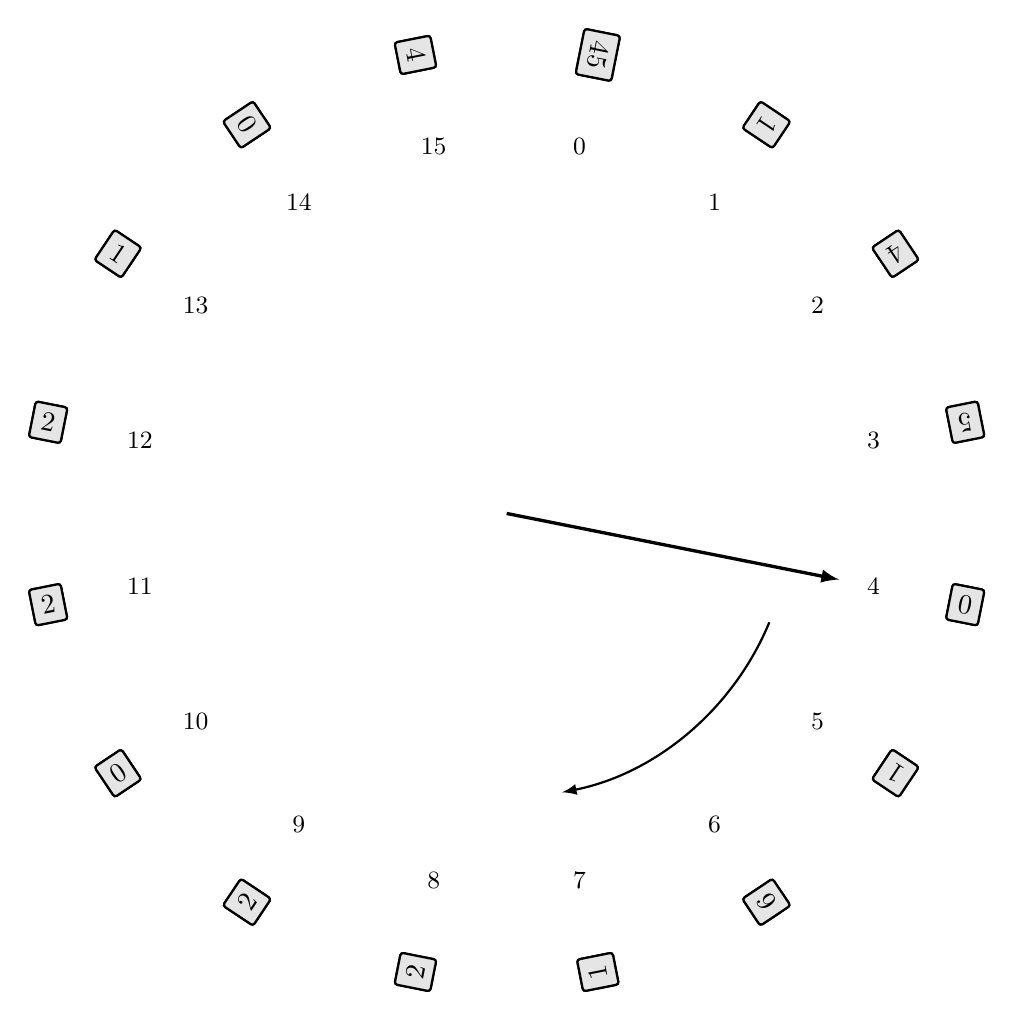
\begin{tikzpicture}
                \foreach \index/\referenced in {0/45, 1/1, 2/4, 3/5, 4/0, 5/1, 6/6, 7/1, 8/2, 9/2, 10/0, 11/2, 12/2, 13/1, 14/0, 15/4} {
                    \ifthenelse{\index < 8}{%
                        \node [refInt, rotate = 90-11.25-\index*22.5] at (90-11.25-\index*22.5:2.5) {\referenced};%
                    }{%
                        \node [refInt, rotate = 270-11.25-\index*22.5] at (90-11.25-\index*22.5:2.5) {\referenced};%
                    }
                    \node [draw = none, font = \small] at (90-11.25-\index*22.5:2) {\index};
                }
                \path[->] (0,0)		edge[hand]		(-11.25:1.8125);
                \draw [->, thick] (0,0)+(-22.5:1.5205) arc [start angle = -22.5, end angle = -78.75, radius = 1.5205];
            \end{tikzpicture}
        }
    \end{minipage}
\end{frame}

\begin{frame}
    \frametitle{Performance Evaluation}

    \pgfplotsset{%
        every axis/.append style = {
            yticklabel style = {font = \scriptsize},
            scaled y ticks = false,
            ybar = .8pt,
            bar width = .225em,
            xmin = -0.75,
            xmax = 7.75,
            xtick style = {draw = none},
            xtick = {0, 1, 2, 3, 4, 5, 6, 7},
            xticklabels = {{\SI{0.1}{\giga\byte}}, {\SI{0.5}{\giga\byte}}, {\SI{1}{\giga\byte}}, {\SI{2.5}{\giga\byte}}, {\SI{5}{\giga\byte}}, {\SI{10}{\giga\byte}}, {\SI{20}{\giga\byte}}, {\SI{30}{\giga\byte}}},
            x tick label style = {align = center,
                                  font = \footnotesize},
            width = .925\textwidth,
            height = .8\paperheight
        }
    }

    \tikzset{%
        fix/.style = {thick, draw = Cerulean!50, fill = Cerulean!25},
        fixfull/.style = {thick, draw = Cerulean, fill = Cerulean!50},
        unfix/.style = {thick, draw = Magenta!50, fill = Magenta!25},
        unfixfull/.style = {thick, draw = Magenta, fill = Magenta!50},
        x2/.style = {dashed},
        missrate/.style = {mark = *}
    }

    \begin{tikzpicture}
        \begin{axis}[ymode = normal,
                     ymin = 0,
                     ymax = 1000000,
                     ymajorgrids = true,
                     yticklabel style = {/pgf/number format/fixed},
                     legend style = {font = \tiny,
                                     legend columns = 4,
                                     /tikz/every even column/.append style = {column sep = 0.05cm},
                                     row sep = -2pt,
                                     draw = none,
                                     fill = none,
                                     at = {(0.5, 0.97)},
                                     anchor = north}]
            \addplot[fix] coordinates
                {(0, 66126.22) (1, 78730.54) (2, 90953.54) (3, 135387.68) (4, 227063.82) (5, 609152.63) (6, 751719.47) (7, 884719.45)};
            \addlegendentry{Fix};
            \addplot[fixfull] coordinates
                {(0, 65393.24) (1, 81024.72) (2, 92649.90) (3, 137824.18) (4, 244067.96) (5, 628208.19) (6, 758292.72) (7, 885172.15)};
            \addlegendentry{FixFull};
            \addplot[unfix] coordinates
                {(0, 67529.88) (1, 80321.59) (2, 94150.54) (3, 144352.48) (4, 246033.75) (5, 621083.97) (6, 761953.84) (7, 885285.05)};
            \addlegendentry{Unfix};
            \addplot[unfixfull] coordinates
                {(0, 66861.31) (1, 86048.74) (2, 95854.25) (3, 139702.65) (4, 251889.60) (5, 648089.89) (6, 760777.46) (7, 882899.51)};
            \addlegendentry{\alert<3->{UnfixFull}};
            \addplot[fix, x2] coordinates
                {(0, 64701.21) (1, 79005.75) (2, 89500.81) (3, 132592.94) (4, 216295.66) (5, 600499.71) (6, 759997.84) (7, 882521.02)};
            \addlegendentry{Fixx2};
            \addplot[fixfull, x2] coordinates
                {(0, 65431.32) (1, 79982.58) (2, 92944.35) (3, 138711.32) (4, 244790.12) (5, 637692.04) (6, 761768.15) (7, 887521.89)};
            \addlegendentry{FixFullx2};
            \addplot[unfix, x2] coordinates
                {(0, 65541.10) (1, 78690.31) (2, 92954.34) (3, 141412.99) (4, 245345.80) (5, 618599.29) (6, 758756.01) (7, 881595.05)};
            \addlegendentry{Unfixx2};
            \addplot[unfixfull, x2] coordinates
                {(0, 65776.77) (1, 83164.87) (2, 95581.74) (3, 143411.60) (4, 262159.61) (5, 651048.14) (6, 773517.04) (7, 890192.98)};
            \addlegendentry{UnfixFullx2};
        \end{axis}
        \begin{axis}[axis y line* = right,
                     ymode = normal,
                     ymin = 100,
                     ymax = 75,
                     grid = none,
                     ycomb = .8pt,
                     y coord trafo/.code = {
                         \pgfmathparse{100 - ####1}
                         \pgfmathresult
                     },
                     yticklabel={\SI[round-mode = places, round-precision = 0]{\tick}{\percent}}]
            \addplot[fix, missrate, xshift = -11.5, visible on = <2->] coordinates
                {(0, 80.11) (1, 88.11) (2, 92.06) (3, 96.37) (4, 98.18) (5, 99.71) (6, 99.85) (7, 99.86)};
            \addplot[fixfull, missrate, xshift = -8.21, visible on = <2->] coordinates
                {(0, 78.99) (1, 87.10) (2, 91.84) (3, 96.29) (4, 98.18) (5, 99.68) (6, 99.85) (7, 99.86)};
            \addplot[unfix, missrate, xshift = -4.93, visible on = <2->] coordinates
                {(0, 79.47) (1, 88.81) (2, 92.39) (3, 96.47) (4, 98.26) (5, 99.71) (6, 99.85) (7, 99.86)};
            \addplot[unfixfull, missrate, xshift = -1.64, visible on = <2->] coordinates
                {(0, 78.12) (1, 87.35) (2, 92.12) (3, 96.33) (4, 98.24) (5, 99.68) (6, 99.85) (7, 99.86)};
            \addplot[fix, x2, missrate, xshift = 1.64, visible on = <2->] coordinates
                {(0, 80.80) (1, 88.50) (2, 92.05) (3, 96.32) (4, 98.16) (5, 99.70) (6, 99.85) (7, 99.86)};
            \addplot[fixfull, x2, missrate, xshift = 4.93, visible on = <2->] coordinates
                {(0, 79.28) (1, 87.19) (2, 91.87) (3, 96.24) (4, 98.16) (5, 99.66) (6, 99.85) (7, 99.86)};
            \addplot[unfix, x2, missrate, xshift = 8.21, visible on = <2->] coordinates
                {(0, 80.47) (1, 89.29) (2, 92.45) (3, 96.51) (4, 98.29) (5, 99.70) (6, 99.85) (7, 99.86)};
            \addplot[unfixfull, x2, missrate, xshift = 11.5, visible on = <2->] coordinates
                {(0, 78.38) (1, 87.74) (2, 92.20) (3, 96.32) (4, 98.26) (5, 99.66) (6, 99.85) (7, 99.86)};
        \end{axis}
    \end{tikzpicture}
\end{frame}

%\subsection[]{Dynamic Generalized CLOCK \cite{Effelsberg:1984}}

%\frame{\subsectionpage}

%\subsubsection[]{DGCLOCK-V1}

%\frame{\subsubsectionpage}

\begin{frame}
    \frametitle{DGCLOCK-V1 Variants}

    \begin{block}{Usage-Count}
        \vspace{-2em}
        \begin{align*}
            \text{(initially)\qquad}\text{UC}\left(p\right) &= F_p\\
            \text{(increase)\qquad}\text{UC}\left(p\right) &= \text{UC}\left(p\right) + R_p\\
            \text{(decrease)\qquad}\text{UC}\left(p\right) &= \text{UC}\left(p\right) - 1
        \end{align*}
        \vspace{-1.5em}
    \end{block}

    \begin{description}
        \item<2->[Fix]          Increase usage-count on \emph{page fix}
        \item<2->[FixFull]      Like \textcolor{structure}{Fix} but also increase usage-count when page cannot be evicted
    \end{description}
    \vspace{.5em}
    \begin{description}
        \item<3->[]     \noindent\begin{minipage}[t]{.225\linewidth}
                            \vspace{-2em}
                            \begin{align*}
                                F_{\text{non-B-tree}} &= 25,\\
                                R_{\text{non-B-tree}} &= 5,
                            \end{align*}
                        \end{minipage}%
                        \noindent\begin{minipage}[t]{.225\linewidth}
                            \vspace{-2em}
                            \begin{align*}
                                F_{\text{root}} &= 25,\\
                                R_{\text{root}} &= 5,
                            \end{align*}\break
                        \end{minipage}%
                        \noindent\begin{minipage}[t]{.225\linewidth}
                            \vspace{-2em}
                            \begin{align*}
                                F_{\text{root} - 1} &= 10,\\
                                R_{\text{root} - 1} &= 2,
                            \end{align*}\break
                        \end{minipage}%
                        \noindent\begin{minipage}[t]{.225\linewidth}
                            \vspace{-2em}
                            \begin{align*}
                                F_{\text{root} - \geq 2} &= 5,\\
                                R_{\text{root} - \geq 2} &= 1
                            \end{align*}
                        \end{minipage}%
                        \vspace{-3em}
        \item<4->[x2]   \noindent\begin{minipage}[t]{.225\linewidth}
                            \vspace{-2em}
                            \begin{align*}
                                F_{\text{non-B-tree}} &= 50,\\
                                R_{\text{non-B-tree}} &= 10,
                            \end{align*}
                            \end{minipage}%
                        \noindent\begin{minipage}[t]{.225\linewidth}
                        \vspace{-2em}
                            \begin{align*}
                                F_{\text{root}} &= 50,\\
                                R_{\text{root}} &= 10,
                            \end{align*}\break
                        \end{minipage}%
                        \noindent\begin{minipage}[t]{.225\linewidth}
                            \vspace{-2em}
                            \begin{align*}
                                F_{\text{root} - 1} &= 25,\\
                                R_{\text{root} - 1} &= 5,
                            \end{align*}\break
                        \end{minipage}%
                        \noindent\begin{minipage}[t]{.225\linewidth}
                            \vspace{-2em}
                            \begin{align*}
                                F_{\text{root} - \geq 2} &= 10,\\
                                R_{\text{root} - \geq 2} &= 2
                            \end{align*}
                        \end{minipage}%
                        \vspace{-3em}
    \end{description}
\end{frame}

\begin{frame}
    \frametitle{Performance Evaluation}

    \pgfplotsset{%
        every axis/.append style = {
            yticklabel style = {font = \scriptsize},
            scaled y ticks = false,
            ybar = .8pt,
            bar width = .5em,
            xmin = -0.75,
            xmax = 7.75,
            xtick style = {draw = none},
            xtick = {0, 1, 2, 3, 4, 5, 6, 7},
            xticklabels = {{\SI{0.1}{\giga\byte}}, {\SI{0.5}{\giga\byte}}, {\SI{1}{\giga\byte}}, {\SI{2.5}{\giga\byte}}, {\SI{5}{\giga\byte}}, {\SI{10}{\giga\byte}}, {\SI{20}{\giga\byte}}, {\SI{30}{\giga\byte}}},
            x tick label style = {align = center,
                                  font = \footnotesize},
            width = .925\textwidth,
            height = .8\paperheight
        }
    }

    \tikzset{%
        fix/.append style = {thick, draw = Cerulean!50, fill = Cerulean!25},
        fixfull/.append style = {thick, draw = Cerulean, fill = Cerulean!50},
        x2/.style = {dashed},
        missrate/.style = {mark = *}
    }

    \begin{tikzpicture}
        \begin{axis}[ymode = normal,
                     ymin = 0,
                     ymax = 1000000,
                     ymajorgrids = true,
                     yticklabel style = {/pgf/number format/fixed},
                     legend style = {font = \tiny,
                                     legend columns = 4,
                                     /tikz/every even column/.append style = {column sep = 0.05cm},
                                     row sep = -2pt,
                                     draw = none,
                                     fill = none,
                                     at = {(0.5, 0.97)},
                                     anchor = north}]
            \addplot[fix] coordinates
                {(0, 66924.04) (1, 79170.81) (2, 90470.43) (3, 124828.87) (4, 183965.95) (5, 387162.61) (6, 690962.18) (7, 883621.85)};
            \addlegendentry{Fix};
            \addplot[fixfull] coordinates
                {(0, 65642.55) (1, 80478.20) (2, 92000.84) (3, 130455.70) (4, 197013.68) (5, 457477.86) (6, 698882.02) (7, 882489.05)};
            \addlegendentry{\alert<4->{FixFull}};
            \addplot[fix, x2, visible on = <2->] coordinates
                {(0, 63997.58) (1, 76973.25) (2, 86599.71) (3, 119294.37) (4, 173211.26) (5, 339305.62) (6, 672246.35) (7, 888587.37)};
            \addlegendentry[visible on = <2->]{Fixx2};
            \addplot[fixfull, x2, visible on = <2->] coordinates
                {(0, 65406.34) (1, 78498.63) (2, 88725.73) (3, 126351.30) (4, 197455.81) (5, 426242.43) (6, 692582.13) (7, 878486.25)};
            \addlegendentry[visible on = <2->]{FixFullx2};
        \end{axis}
        \begin{axis}[axis y line* = right,
                     ymode = normal,
                     ymin = 100,
                     ymax = 75,
                     grid = none,
                     ycomb = .8pt,
                     y coord trafo/.code = {
                         \pgfmathparse{100 - ####1}
                         \pgfmathresult
                     },
                     yticklabel={\SI[round-mode = places, round-precision = 0]{\tick}{\percent}}]
            \addplot[fix, missrate, xshift = -9.5, visible on = <3->] coordinates
                {(0, 82.53) (1, 89.69) (2, 91.99) (3, 95.93) (4, 97.77) (5, 99.43) (6, 99.84) (7, 99.86)};
            \addplot[fixfull, missrate, xshift = -3.167, visible on = <3->] coordinates
                {(0, 81.31) (1, 89.66) (2, 92.16) (3, 96.04) (4, 97.83) (5, 99.45) (6, 99.84) (7, 99.86)};
            \addplot[fix, x2, missrate, xshift = 3.167, visible on = <3->] coordinates
                {(0, 83.70) (1, 89.65) (2, 91.88) (3, 95.87) (4, 97.78) (5, 99.44) (6, 99.84) (7, 99.86)};
            \addplot[fixfull, x2, missrate, xshift = 9.5, visible on = <3->] coordinates
                {(0, 82.11) (1, 89.73) (2, 92.10) (3, 95.98) (4, 97.87) (5, 99.44) (6, 99.84) (7, 99.86)};
        \end{axis}
    \end{tikzpicture}
\end{frame}

%\subsubsection[]{DGCLOCK-V2}

%\frame{\subsubsectionpage}

\begin{frame}
    \frametitle{DGCLOCK-V2 Variants}

    \begin{block}<2->{Usage-Count}
        \vspace{-2em}
        \begin{align*}
            \text{(initially)\qquad}\text{UC}\left(p\right) &= F_p\\
            \text{(set)\qquad}\text{UC}\left(p\right) &= R_p\\
            \text{(decrease)\qquad}\text{UC}\left(p\right) &= \text{UC}\left(p\right) - 1
        \end{align*}
        \vspace{-1.5em}
    \end{block}

    \begin{description}
        \item[Fix]          Set usage-count on \emph{page fix}
        \item[FixFull]      Like \textcolor{structure}{Fix} but also set usage-count when page cannot be evicted
    \end{description}
    \vspace{.5em}
    \begin{description}
        \item[]     \noindent\begin{minipage}[t]{.225\linewidth}
                        \vspace{-2em}
                        \begin{align*}
                            F_{\text{non-B-tree}} &= 25,\\
                            R_{\text{non-B-tree}} &= 5,
                        \end{align*}
                    \end{minipage}%
                    \noindent\begin{minipage}[t]{.225\linewidth}
                        \vspace{-2em}
                        \begin{align*}
                            F_{\text{root}} &= 25,\\
                            R_{\text{root}} &= 5,
                        \end{align*}\break
                    \end{minipage}%
                    \noindent\begin{minipage}[t]{.225\linewidth}
                        \vspace{-2em}
                        \begin{align*}
                            F_{\text{root} - 1} &= 10,\\
                            R_{\text{root} - 1} &= 2,
                        \end{align*}\break
                    \end{minipage}%
                    \noindent\begin{minipage}[t]{.225\linewidth}
                        \vspace{-2em}
                        \begin{align*}
                            F_{\text{root} - \geq 2} &= 5,\\
                            R_{\text{root} - \geq 2} &= 1
                        \end{align*}
                    \end{minipage}%
                    \vspace{-3em}
        \item[x2]   \noindent\begin{minipage}[t]{.225\linewidth}
                        \vspace{-2em}
                        \begin{align*}
                            F_{\text{non-B-tree}} &= 50,\\
                            R_{\text{non-B-tree}} &= 10,
                        \end{align*}
                    \end{minipage}%
                    \noindent\begin{minipage}[t]{.225\linewidth}
                        \vspace{-2em}
                        \begin{align*}
                            F_{\text{root}} &= 50,\\
                            R_{\text{root}} &= 10,
                        \end{align*}\break
                    \end{minipage}%
                    \noindent\begin{minipage}[t]{.225\linewidth}
                        \vspace{-2em}
                        \begin{align*}
                            F_{\text{root} - 1} &= 25,\\
                            R_{\text{root} - 1} &= 5,
                        \end{align*}\break
                    \end{minipage}%
                    \noindent\begin{minipage}[t]{.225\linewidth}
                        \vspace{-2em}
                        \begin{align*}
                            F_{\text{root} - \geq 2} &= 10,\\
                            R_{\text{root} - \geq 2} &= 2
                        \end{align*}
                    \end{minipage}%
                    \vspace{-3em}
    \end{description}
\end{frame}

\begin{frame}
    \frametitle{Performance Evaluation}

    \pgfplotsset{%
        every axis/.append style = {
            yticklabel style = {font = \scriptsize},
            scaled y ticks = false,
            ybar = .8pt,
            bar width = .5em,
            xmin = -0.75,
            xmax = 7.75,
            xtick style = {draw = none},
            xtick = {0, 1, 2, 3, 4, 5, 6, 7},
            xticklabels = {{\SI{0.1}{\giga\byte}}, {\SI{0.5}{\giga\byte}}, {\SI{1}{\giga\byte}}, {\SI{2.5}{\giga\byte}}, {\SI{5}{\giga\byte}}, {\SI{10}{\giga\byte}}, {\SI{20}{\giga\byte}}, {\SI{30}{\giga\byte}}},
            x tick label style = {align = center,
                                  font = \footnotesize},
            width = .925\textwidth,
            height = .8\paperheight
        }
    }

    \tikzset{%
        fix/.append style = {thick, draw = Cerulean!50, fill = Cerulean!25},
        fixfull/.append style = {thick, draw = Cerulean, fill = Cerulean!50},
        x2/.style = {dashed},
        missrate/.style = {mark = *}
    }

    \begin{tikzpicture}
        \begin{axis}[ymode = normal,
                     ymin = 0,
                     ymax = 1000000,
                     ymajorgrids = true,
                     yticklabel style = {/pgf/number format/fixed},
                     legend style = {font = \tiny,
                                     legend columns = 4,
                                     /tikz/every even column/.append style = {column sep = 0.05cm},
                                     row sep = -2pt,
                                     draw = none,
                                     fill = none,
                                     at = {(0.5, 0.97)},
                                     anchor = north}]
            \addplot[fix] coordinates
                {(0, 65328.91) (1, 85150.60) (2, 89698.46) (3, 136511.50) (4, 223061.99) (5, 620475.67) (6, 761789.06) (7, 889050.53)};
            \addlegendentry{Fix};
            \addplot[fixfull] coordinates
                {(0, 66091.61) (1, 80892.64) (2, 92705.83) (3, 138269.21) (4, 242778.79) (5, 627736.54) (6, 758085.38) (7, 884485.20)};
            \addlegendentry{\alert<3->{FixFull}};
            \addplot[fix, x2] coordinates
                {(0, 63105.93) (1, 76825.59) (2, 86478.06) (3, 132019.39) (4, 216118.93) (5, 586734.37) (6, 750078.00) (7, 891430.09)};
            \addlegendentry{Fixx2};
            \addplot[fixfull, x2] coordinates
                {(0, 67430.20) (1, 82767.14) (2, 93595.51) (3, 134557.05) (4, 241585.52) (5, 623190.59) (6, 760453.26) (7, 882858.20)};
            \addlegendentry{FixFullx2};
        \end{axis}
        \begin{axis}[axis y line* = right,
                     ymode = normal,
                     ymin = 100,
                     ymax = 75,
                     grid = none,
                     ycomb = .8pt,
                     y coord trafo/.code = {
                         \pgfmathparse{100 - ####1}
                         \pgfmathresult
                     },
                     yticklabel={\SI[round-mode = places, round-precision = 0]{\tick}{\percent}}]
            \addplot[fix, missrate, xshift = -9.5, visible on = <2->] coordinates
                {(0, 80.69) (1, 88.79) (2, 92.25) (3, 96.38) (4, 98.18) (5, 99.71) (6, 99.85) (7, 99.86)};
            \addplot[fixfull, missrate, xshift = -3.167, visible on = <2->] coordinates
                {(0, 79.73) (1, 87.87) (2, 92.21) (3, 96.31) (4, 98.18) (5, 99.68) (6, 99.85) (7, 99.86)};
            \addplot[fix, x2, missrate, xshift = 3.167, visible on = <2->] coordinates
                {(0, 81.53) (1, 89.24) (2, 92.22) (3, 96.37) (4, 98.19) (5, 99.73) (6, 99.85) (7, 99.86)};
            \addplot[fixfull, x2, missrate, xshift = 9.5, visible on = <2->] coordinates
                {(0, 80.17) (1, 88.28) (2, 92.31) (3, 96.30) (4, 98.17) (5, 99.69) (6, 99.85) (7, 99.86)};
        \end{axis}
    \end{tikzpicture}
\end{frame}

%\subsection[]{Least Reference Density \cite{Effelsberg:1984}}

%\frame{\subsectionpage}

%\subsubsection[]{LRD-V1}

%\frame{\subsubsectionpage}

%\subsubsection[]{LRD-V2}

%\frame{\subsubsectionpage}

\begin{frame}
    \frametitle{LRD-V2 Variants}

    \begin{block}{Reference Counts}
        \vspace{-2em}
        \begin{align*}
            \text{(aging)\qquad}\text{UC}\left(p\right) &= \text{UC}\left(p\right) \circ x\\
            \text{(increase)\qquad}\text{RC}\left(p\right) &= \text{RC}\left(p\right) + 1
        \end{align*}
        \vspace{-1.5em}
    \end{block}

    \begin{description}
        \item<2->[$f \circ x$]  Perform aging (using $\circ x$) on each reference count every $f \cdot \text{bufferPoolSize}$ global page references
    \end{description}
\end{frame}

\begin{frame}
    \frametitle{Performance Evaluation I}

    \pgfplotsset{%
        every axis/.append style = {
            yticklabel style = {font = \scriptsize},
            scaled y ticks = false,
            ybar = .8pt,
            bar width = .1em,
            xmin = -0.5,
            xmax = 3.5,
            xtick style = {draw = none},
            xtick = {0, 1, 2, 3, 4, 5, 6, 7},
            xticklabels = {{\SI{0.1}{\giga\byte}}, {\SI{0.5}{\giga\byte}}, {\SI{1}{\giga\byte}}, {\SI{2.5}{\giga\byte}}, {\SI{5}{\giga\byte}}, {\SI{10}{\giga\byte}}, {\SI{20}{\giga\byte}}, {\SI{30}{\giga\byte}}},
            x tick label style = {align = center,
                font = \footnotesize},
            width = .95\textwidth,
            height = .8\paperheight
        }
    }

    \tikzset{%
        aging1/.style = {thin, solid},
        aging2/.style = {thin, densely dotted},
        aging5/.style = {thin, dotted},
        aging10/.style = {thin, loosely dotted},
        factor10/.style = {thin, draw = Cerulean, fill = Cerulean!10},
        factor25/.style = {thin, draw = Cerulean, fill = Cerulean!25},
        factor50/.style = {thin, draw = Cerulean, fill = Cerulean!50},
        factor75/.style = {thin, draw = Cerulean, fill = Cerulean!75},
        subtractor1/.style = {thin, draw = Magenta, fill = Magenta!10},
        subtractor2/.style = {thin, draw = Magenta, fill = Magenta!25},
        subtractor5/.style = {thin, draw = Magenta, fill = Magenta!50},
        subtractor10/.style = {thin, draw = Magenta, fill = Magenta!75},
        missrate/.style = {mark = *}
    }

    \centering
    \begin{tikzpicture}
        \begin{axis}[ymode = normal,
                     ymin = 0,
                     ymax = 35000,
                     ytick distance = 5000,
                     ymajorgrids = true,
                     yticklabel style = {/pgf/number format/fixed},
                     legend style = {font = \tiny,
                                     legend columns = 5,
                                     /tikz/every even column/.append style = {column sep = 0.05cm},
                                     row sep = -2pt,
                                     draw = none,
                                     fill = none,
                                     at = {(0.99, 0.99)},
                                     anchor = north east}]
            \addplot[aging1, factor10] coordinates
                {(0, 21406.28) (1, 12650.43) (2, 11952.45) (3, 13316.72) (4, 21335.30) (5, 107604.30) (6, 560356.44) (7, 881206.84)};
            \addlegendentry{$1 \cdot 0.1$};
            \addplot[aging1, factor25] coordinates
                {(0, 21229.56) (1, 13326.91) (2, 12221.95) (3, 13649.17) (4, 21819.81) (5, 108729.86) (6, 561166.91) (7, 885438.97)};
            \addlegendentry{$1 \cdot 0.25$};
            \addplot[aging1, factor50] coordinates
                {(0, 21185.92) (1, 13601.06) (2, 12296.55) (3, 13787.22) (4, 22244.46) (5, 109129.91) (6, 561073.82) (7, 885928.79)};
            \addlegendentry{$1 \cdot 0.5$};
            \addplot[aging1, factor75] coordinates
                {(0, 21406.10) (1, 13600.25) (2, 12264.08) (3, 13687.78) (4, 22212.46) (5, 102558.02) (6, 556181.11) (7, 870721.84)};
            \addlegendentry{$1 \cdot 0.75$};
            \addplot[aging2, factor10, visible on = <2->] coordinates
                {(0, 24572.00) (1, 12830.88) (2, 11955.41) (3, 14865.22) (4, 23863.07) (5, 110799.80) (6, 553862.83) (7, 881440.46)};
            \addlegendentry[visible on = <2->]{$2 \cdot 0.1$};
            \addplot[aging2, factor25, visible on = <2->] coordinates
                {(0, 24879.11) (1, 12632.71) (2, 12230.80) (3, 14606.87) (4, 23560.41) (5, 108607.90) (6, 563009.63) (7, 877781.04)};
            \addlegendentry[visible on = <2->]{$2 \cdot 0.25$};
            \addplot[aging2, factor50, visible on = <2->] coordinates
                {(0, 27463.08) (1, 13488.06) (2, 11876.03) (3, 14737.48) (4, 23234.38) (5, 104864.03) (6, 564491.24) (7, 884524.59)};
            \addlegendentry[visible on = <2->]{$2 \cdot 0.5$};
            \addplot[aging2, factor75, visible on = <2->] coordinates
                {(0, 26750.60) (1, 14230.10) (2, 11339.76) (3, 14391.62) (4, 22197.42) (5, 98365.75) (6, 565206.94) (7, 871683.63)};
            \addlegendentry[visible on = <2->]{$2 \cdot 0.75$};
            \addplot[aging5, factor10, visible on = <3->] coordinates
                {(0, 24696.72) (1, 20672.13) (2, 13931.04) (3, 16492.65) (4, 24195.56) (5, 104128.34) (6, 565566.58) (7, 875879.67)};
            \addlegendentry[visible on = <3->]{$5 \cdot 0.1$};
            \addplot[aging5, factor25, visible on = <3->] coordinates
                {(0, 24382.79) (1, 21142.77) (2, 13901.25) (3, 16197.79) (4, 23286.67) (5, 101415.07) (6, 566554.44) (7, 854237.82)};
            \addlegendentry[visible on = <3->]{$5 \cdot 0.25$};
            \addplot[aging5, factor50, visible on = <3->] coordinates
                {(0, 22172.58) (1, 22288.41) (2, 16183.10) (3, 15071.92) (4, 22709.92) (5, 101311.56) (6, 568668.60) (7, 885584.98)};
            \addlegendentry[visible on = <3->]{$5 \cdot 0.5$};
            \addplot[aging5, factor75, visible on = <3->] coordinates
                {(0, 19933.19) (1, 21803.43) (2, 16054.33) (3, 14855.02) (4, 21838.90) (5, 101383.15) (6, 567983.31) (7, 879927.67)};
            \addlegendentry[visible on = <3->]{$5 \cdot 0.75$};
            \addplot[aging10, factor10, visible on = <4->] coordinates
                {(0, 21173.57) (1, 16567.32) (2, 16107.05) (3, 16328.90) (4, 23275.65) (5, 101983.20) (6, 568949.10) (7, 873542.37)};
            \addlegendentry[visible on = <4->]{$10 \cdot 0.1$};
            \addplot[aging10, factor25, visible on = <4->] coordinates
                {(0, 21156.93) (1, 17045.94) (2, 14692.11) (3, 15843.30) (4, 23641.94) (5, 104729.69) (6, 570153.19) (7, 886153.35)};
            \addlegendentry[visible on = <4->]{$10 \cdot 0.25$};
            \addplot[aging10, factor50, visible on = <4->] coordinates
                {(0, 20030.21) (1, 15300.29) (2, 14298.09) (3, 17998.28) (4, 22874.09) (5, 104934.56) (6, 568896.82) (7, 883188.29)};
            \addlegendentry[visible on = <4->]{$10 \cdot 0.5$};
            \addplot[aging10, factor75, visible on = <4->] coordinates
                {(0, 18804.73) (1, 14373.60) (2, 11860.91) (3, 16238.28) (4, 23661.79) (5, 104948.84) (6, 565246.06) (7, 875551.76)};
            \addlegendentry[visible on = <4->]{$10 \cdot 0.75$};
            \addplot[aging1, subtractor1, visible on = <5->] coordinates
                {(0, 22205.54) (1, 13689.20) (2, 11647.54) (3, 13185.03) (4, 21379.10) (5, 97095.02) (6, 561065.43) (7, 880034.75)};
            \addlegendentry[visible on = <5->]{$1 - 1$};
            \addplot[aging2, subtractor1, visible on = <6->] coordinates
                {(0, 25875.37) (1, 15068.35) (2, 11055.92) (3, 13782.20) (4, 21574.34) (5, 94173.80) (6, 564336.97) (7, 884591.21)};
            \addlegendentry[visible on = <6->]{$2 - 1$};
            \addplot[aging2, subtractor2, visible on = <6->] coordinates
                {(0, 25580.63) (1, 13411.26) (2, 11569.42) (3, 14101.23) (4, 22484.10) (5, 95574.59) (6, 563649.76) (7, 881626.44)};
            \addlegendentry[visible on = <6->]{$2 - 2$};
            \addplot[aging5, subtractor1, visible on = <7->] coordinates
                {(0, 19443.53) (1, 19042.59) (2, 16121.09) (3, 15401.18) (4, 21869.28) (5, 100206.75) (6, 564463.74) (7, 883677.31)};
            \addlegendentry[visible on = <7->]{$5 - 1$};
            \addplot[aging5, subtractor2, visible on = <7->] coordinates
                {(0, 21102.07) (1, 19626.83) (2, 15214.51) (3, 15101.12) (4, 21829.08) (5, 97110.92) (6, 566692.17) (7, 883334.89)};
            \addlegendentry[visible on = <7->]{$5 - 2$};
            \addplot[aging5, subtractor5, visible on = <7->] coordinates
                {(0, 24105.29) (1, 21103.78) (2, 14121.79) (3, 15354.45) (4, 22721.14) (5, 96840.11) (6, 564948.52) (7, 872378.13)};
            \addlegendentry[visible on = <7->]{$5 - 5$};
            \addplot[aging10, subtractor1, visible on = <8->] coordinates
                {(0, 18399.98) (1, 14784.47) (2, 11864.11) (3, 18062.91) (4, 24726.77) (5, 102036.64) (6, 560973.13) (7, 872965.49)};
            \addlegendentry[visible on = <8->]{$10 - 1$};
            \addplot[aging10, subtractor2, visible on = <8->] coordinates
                {(0, 19053.14) (1, 15259.32) (2, 12963.87) (3, 14831.29) (4, 21873.20) (5, 101063.13) (6, 566213.23) (7, 886027.09)};
            \addlegendentry[visible on = <8->]{$10 - 2$};
            \addplot[aging10, subtractor5, visible on = <8->] coordinates
                {(0, 20043.86) (1, 16215.95) (2, 14761.69) (3, 15769.38) (4, 22440.64) (5, 97994.19) (6, 569786.60) (7, 876719.18)};
            \addlegendentry[visible on = <8->]{$10 - 5$};
            \addplot[aging10, subtractor10, visible on = <8->] coordinates
                {(0, 20975.98) (1, 16271.13) (2, 15646.43) (3, 16410.83) (4, 22705.13) (5, 98975.93) (6, 567759.95) (7, 890394.41)};
            \addlegendentry[visible on = <8->]{$10 - 10$};
        \end{axis}
        \begin{axis}[axis y line* = right,
                     ymode = normal,
                     ymin = 100,
                     ymax = 65,
                     ytick distance = 5,
                     grid = none,
                     ycomb = .8pt,
                     y coord trafo/.code = {
                         \pgfmathparse{100 - ####1}
                         \pgfmathresult
                     },
                     yticklabel={\SI[round-mode = places, round-precision = 0]{\tick}{\percent}}]
            \addplot[aging1, factor10, missrate, xshift = 23.675*(-25/25), visible on = <9->] coordinates
                {(0, 80.00) (1, 86.88) (2, 90.01) (3, 94.22) (4, 97.40) (5, 99.48) (6, 99.83) (7, 99.86)};
            \addplot[aging1, factor25, missrate, xshift = 23.675*(-23/25), visible on = <9->] coordinates
                {(0, 80.25) (1, 87.37) (2, 90.34) (3, 94.30) (4, 97.44) (5, 99.48) (6, 99.83) (7, 99.86)};
            \addplot[aging1, factor50, missrate, xshift = 23.675*(-21/25), visible on = <9->] coordinates
                {(0, 80.97) (1, 88.40) (2, 90.87) (3, 94.57) (4, 97.56) (5, 99.48) (6, 99.83) (7, 99.86)};
            \addplot[aging1, factor75, missrate, xshift = 23.675*(-19/25), visible on = <9->] coordinates
                {(0, 81.33) (1, 88.82) (2, 91.02) (3, 94.63) (4, 97.57) (5, 99.46) (6, 99.83) (7, 99.86)};
            \addplot[aging2, factor10, missrate, xshift = 23.675*(-17/25), visible on = <9->] coordinates
                {(0, 81.31) (1, 88.23) (2, 91.48) (3, 95.12) (4, 97.67) (5, 99.48) (6, 99.83) (7, 99.86)};
            \addplot[aging2, factor25, missrate, xshift = 23.675*(-15/25), visible on = <9->] coordinates
                {(0, 81.66) (1, 88.75) (2, 91.61) (3, 95.17) (4, 97.69) (5, 99.47) (6, 99.83) (7, 99.86)};
            \addplot[aging2, factor50, missrate, xshift = 23.675*(-13/25), visible on = <9->] coordinates
                {(0, 82.53) (1, 89.31) (2, 92.02) (3, 95.52) (4, 97.73) (5, 99.46) (6, 99.83) (7, 99.86)};
            \addplot[aging2, factor75, missrate, xshift = 23.675*(-11/25), visible on = <9->] coordinates
                {(0, 82.56) (1, 89.52) (2, 92.11) (3, 95.59) (4, 97.73) (5, 99.43) (6, 99.83) (7, 99.86)};
            \addplot[aging5, factor10, missrate, xshift = 23.675*(-9/25), visible on = <9->] coordinates
                {(0, 82.23) (1, 89.32) (2, 92.26) (3, 96.06) (4, 97.76) (5, 99.45) (6, 99.83) (7, 99.86)};
            \addplot[aging5, factor25, missrate, xshift = 23.675*(-7/25), visible on = <9->] coordinates
                {(0, 82.26) (1, 89.48) (2, 92.32) (3, 96.10) (4, 97.77) (5, 99.44) (6, 99.83) (7, 99.86)};
            \addplot[aging5, factor50, missrate, xshift = 23.675*(-5/25), visible on = <9->] coordinates
                {(0, 82.14) (1, 89.59) (2, 92.34) (3, 96.26) (4, 97.81) (5, 99.44) (6, 99.83) (7, 99.86)};
            \addplot[aging5, factor75, missrate, xshift = 23.675*(-3/25), visible on = <9->] coordinates
                {(0, 81.86) (1, 89.67) (2, 92.32) (3, 96.29) (4, 97.82) (5, 99.45) (6, 99.83) (7, 99.86)};
            \addplot[aging10, factor10, missrate, xshift = 23.675*(-1/25), visible on = <9->] coordinates
                {(0, 82.13) (1, 89.33) (2, 92.27) (3, 96.23) (4, 97.81) (5, 99.44) (6, 99.83) (7, 99.86)};
            \addplot[aging10, factor25, missrate, xshift = 23.675*(1/25), visible on = <9->] coordinates
                {(0, 82.01) (1, 89.47) (2, 92.29) (3, 96.23) (4, 97.86) (5, 99.44) (6, 99.83) (7, 99.86)};
            \addplot[aging10, factor50, missrate, xshift = 23.675*(3/25), visible on = <9->] coordinates
                {(0, 81.90) (1, 89.49) (2, 92.30) (3, 96.32) (4, 97.92) (5, 99.46) (6, 99.83) (7, 99.86)};
            \addplot[aging10, factor75, missrate, xshift = 23.675*(5/25), visible on = <9->] coordinates
                {(0, 81.53) (1, 89.54) (2, 92.25) (3, 96.31) (4, 97.95) (5, 99.48) (6, 99.83) (7, 99.86)};
            \addplot[aging1, subtractor1, missrate, xshift = 23.675*(7/25), visible on = <9->] coordinates
                {(0, 81.78) (1, 89.05) (2, 91.01) (3, 94.54) (4, 97.49) (5, 99.41) (6, 99.83) (7, 99.86)};
            \addplot[aging2, subtractor1, missrate, xshift = 23.675*(9/25), visible on = <9->] coordinates
                {(0, 82.83) (1, 89.40) (2, 91.94) (3, 95.50) (4, 97.69) (5, 99.42) (6, 99.83) (7, 99.86)};
            \addplot[aging2, subtractor2, missrate, xshift = 23.675*(11/25), visible on = <9->] coordinates
                {(0, 82.35) (1, 89.36) (2, 91.71) (3, 95.14) (4, 97.63) (5, 99.41) (6, 99.83) (7, 99.86)};
            \addplot[aging5, subtractor1, missrate, xshift = 23.675*(13/25), visible on = <9->] coordinates
                {(0, 81.64) (1, 89.42) (2, 91.91) (3, 96.25) (4, 97.85) (5, 99.46) (6, 99.83) (7, 99.86)};
            \addplot[aging5, subtractor2, missrate, xshift = 23.675*(15/25), visible on = <9->] coordinates
                {(0, 81.89) (1, 89.43) (2, 91.94) (3, 96.11) (4, 97.74) (5, 99.43) (6, 99.83) (7, 99.86)};
            \addplot[aging5, subtractor5, missrate, xshift = 23.675*(17/25), visible on = <9->] coordinates
                {(0, 82.47) (1, 89.53) (2, 92.10) (3, 96.00) (4, 97.70) (5, 99.42) (6, 99.83) (7, 99.86)};
            \addplot[aging10, subtractor1, missrate, xshift = 23.675*(19/25), visible on = <9->] coordinates
                {(0, 81.35) (1, 89.43) (2, 92.05) (3, 96.25) (4, 97.99) (5, 99.47) (6, 99.83) (7, 99.86)};
            \addplot[aging10, subtractor2, missrate, xshift = 23.675*(21/25), visible on = <9->] coordinates
                {(0, 81.67) (1, 89.42) (2, 92.02) (3, 96.22) (4, 97.87) (5, 99.46) (6, 99.83) (7, 99.86)};
            \addplot[aging10, subtractor5, missrate, xshift = 23.675*(23/25), visible on = <9->] coordinates
                {(0, 81.91) (1, 89.46) (2, 92.01) (3, 96.12) (4, 97.78) (5, 99.43) (6, 99.83) (7, 99.86)};
            \addplot[aging10, subtractor10, missrate, xshift = 23.675*(25/25), visible on = <9->] coordinates
                {(0, 82.17) (1, 89.48) (2, 92.10) (3, 96.14) (4, 97.77) (5, 99.43) (6, 99.83) (7, 99.86)};
        \end{axis}
    \end{tikzpicture}
\end{frame}

\begin{frame}
    \frametitle{Performance Evaluation II}

    \pgfplotsset{%
        every axis/.append style = {
            scaled y ticks = false,
            ybar = .8pt,
            bar width = .1em,
            xmin = 3.5,
            xmax = 7.5,
            xtick style = {draw = none},
            xtick = {0, 1, 2, 3, 4, 5, 6, 7},
            xticklabels = {{\SI{0.1}{\giga\byte}}, {\SI{0.5}{\giga\byte}}, {\SI{1}{\giga\byte}}, {\SI{2.5}{\giga\byte}}, {\SI{5}{\giga\byte}}, {\SI{10}{\giga\byte}}, {\SI{20}{\giga\byte}}, {\SI{30}{\giga\byte}}},
            x tick label style = {align = center,
                font = \footnotesize},
            width = .95\textwidth,
            height = .8\paperheight
        }
    }

    \tikzset{%
        aging1/.style = {thin, solid},
        aging2/.style = {thin, densely dotted},
        aging5/.style = {thin, dotted},
        aging10/.style = {thin, loosely dotted},
        factor10/.style = {thin, draw = Cerulean, fill = Cerulean!10},
        factor25/.style = {thin, draw = Cerulean, fill = Cerulean!25},
        factor50/.style = {thin, draw = Cerulean, fill = Cerulean!50},
        factor75/.style = {thin, draw = Cerulean, fill = Cerulean!75},
        subtractor1/.style = {thin, draw = Magenta, fill = Magenta!10},
        subtractor2/.style = {thin, draw = Magenta, fill = Magenta!25},
        subtractor5/.style = {thin, draw = Magenta, fill = Magenta!50},
        subtractor10/.style = {thin, draw = Magenta, fill = Magenta!75},
        missrate/.style = {mark = *}
    }

    \centering
    \begin{tikzpicture}
        \begin{axis}[ymode = normal,
                     ymin = 0,
                     ymax = 1500000,
                     ytick distance = 250000,
                     ymajorgrids = true,
                     yticklabel style = {/pgf/number format/fixed},
                     legend style = {font = \tiny,
                                     legend columns = 4,
                                     /tikz/every even column/.append style = {column sep = 0.05cm},
                                     row sep = -2pt,
                                     draw = none,
                                     fill = none,
                                     at = {(0.525, 0.99)},
                                     anchor = north}]
            \addplot[aging1, factor10] coordinates
                {(0, 21406.28) (1, 12650.43) (2, 11952.45) (3, 13316.72) (4, 21335.30) (5, 107604.30) (6, 560356.44) (7, 881206.84)};
            \addlegendentry{$1 \cdot 0.1$};
            \addplot[aging1, factor25] coordinates
                {(0, 21229.56) (1, 13326.91) (2, 12221.95) (3, 13649.17) (4, 21819.81) (5, 108729.86) (6, 561166.91) (7, 885438.97)};
            \addlegendentry{$1 \cdot 0.25$};
            \addplot[aging1, factor50] coordinates
                {(0, 21185.92) (1, 13601.06) (2, 12296.55) (3, 13787.22) (4, 22244.46) (5, 109129.91) (6, 561073.82) (7, 885928.79)};
            \addlegendentry{$1 \cdot 0.5$};
            \addplot[aging1, factor75] coordinates
                {(0, 21406.10) (1, 13600.25) (2, 12264.08) (3, 13687.78) (4, 22212.46) (5, 102558.02) (6, 556181.11) (7, 870721.84)};
            \addlegendentry{$1 \cdot 0.75$};
            \addplot[aging2, factor10, visible on = <2->] coordinates
                {(0, 24572.00) (1, 12830.88) (2, 11955.41) (3, 14865.22) (4, 23863.07) (5, 110799.80) (6, 553862.83) (7, 881440.46)};
            \addlegendentry[visible on = <2->]{$2 \cdot 0.1$};
            \addplot[aging2, factor25, visible on = <2->] coordinates
                {(0, 24879.11) (1, 12632.71) (2, 12230.80) (3, 14606.87) (4, 23560.41) (5, 108607.90) (6, 563009.63) (7, 877781.04)};
            \addlegendentry[visible on = <2->]{$2 \cdot 0.25$};
            \addplot[aging2, factor50, visible on = <2->] coordinates
                {(0, 27463.08) (1, 13488.06) (2, 11876.03) (3, 14737.48) (4, 23234.38) (5, 104864.03) (6, 564491.24) (7, 884524.59)};
            \addlegendentry[visible on = <2->]{$2 \cdot 0.5$};
            \addplot[aging2, factor75, visible on = <2->] coordinates
                {(0, 26750.60) (1, 14230.10) (2, 11339.76) (3, 14391.62) (4, 22197.42) (5, 98365.75) (6, 565206.94) (7, 871683.63)};
            \addlegendentry[visible on = <2->]{$2 \cdot 0.75$};
            \addplot[aging5, factor10, visible on = <3->] coordinates
                {(0, 24696.72) (1, 20672.13) (2, 13931.04) (3, 16492.65) (4, 24195.56) (5, 104128.34) (6, 565566.58) (7, 875879.67)};
            \addlegendentry[visible on = <3->]{$5 \cdot 0.1$};
            \addplot[aging5, factor25, visible on = <3->] coordinates
                {(0, 24382.79) (1, 21142.77) (2, 13901.25) (3, 16197.79) (4, 23286.67) (5, 101415.07) (6, 566554.44) (7, 854237.82)};
            \addlegendentry[visible on = <3->]{$5 \cdot 0.25$};
            \addplot[aging5, factor50, visible on = <3->] coordinates
                {(0, 22172.58) (1, 22288.41) (2, 16183.10) (3, 15071.92) (4, 22709.92) (5, 101311.56) (6, 568668.60) (7, 885584.98)};
            \addlegendentry[visible on = <3->]{$5 \cdot 0.5$};
            \addplot[aging5, factor75, visible on = <3->] coordinates
                {(0, 19933.19) (1, 21803.43) (2, 16054.33) (3, 14855.02) (4, 21838.90) (5, 101383.15) (6, 567983.31) (7, 879927.67)};
            \addlegendentry[visible on = <3->]{$5 \cdot 0.75$};
            \addplot[aging10, factor10, visible on = <4->] coordinates
                {(0, 21173.57) (1, 16567.32) (2, 16107.05) (3, 16328.90) (4, 23275.65) (5, 101983.20) (6, 568949.10) (7, 873542.37)};
            \addlegendentry[visible on = <4->]{$10 \cdot 0.1$};
            \addplot[aging10, factor25, visible on = <4->] coordinates
                {(0, 21156.93) (1, 17045.94) (2, 14692.11) (3, 15843.30) (4, 23641.94) (5, 104729.69) (6, 570153.19) (7, 886153.35)};
            \addlegendentry[visible on = <4->]{$10 \cdot 0.25$};
            \addplot[aging10, factor50, visible on = <4->] coordinates
                {(0, 20030.21) (1, 15300.29) (2, 14298.09) (3, 17998.28) (4, 22874.09) (5, 104934.56) (6, 568896.82) (7, 883188.29)};
            \addlegendentry[visible on = <4->]{$10 \cdot 0.5$};
            \addplot[aging10, factor75, visible on = <4->] coordinates
                {(0, 18804.73) (1, 14373.60) (2, 11860.91) (3, 16238.28) (4, 23661.79) (5, 104948.84) (6, 565246.06) (7, 875551.76)};
            \addlegendentry[visible on = <4->]{$10 \cdot 0.75$};
            \addplot[aging1, subtractor1, visible on = <5->] coordinates
                {(0, 22205.54) (1, 13689.20) (2, 11647.54) (3, 13185.03) (4, 21379.10) (5, 97095.02) (6, 561065.43) (7, 880034.75)};
            \addlegendentry[visible on = <5->]{$1 - 1$};
            \addplot[aging2, subtractor1, visible on = <6->] coordinates
                {(0, 25875.37) (1, 15068.35) (2, 11055.92) (3, 13782.20) (4, 21574.34) (5, 94173.80) (6, 564336.97) (7, 884591.21)};
            \addlegendentry[visible on = <6->]{$2 - 1$};
            \addplot[aging2, subtractor2, visible on = <6->] coordinates
                {(0, 25580.63) (1, 13411.26) (2, 11569.42) (3, 14101.23) (4, 22484.10) (5, 95574.59) (6, 563649.76) (7, 881626.44)};
            \addlegendentry[visible on = <6->]{$2 - 2$};
            \addplot[aging5, subtractor1, visible on = <7->] coordinates
                {(0, 19443.53) (1, 19042.59) (2, 16121.09) (3, 15401.18) (4, 21869.28) (5, 100206.75) (6, 564463.74) (7, 883677.31)};
            \addlegendentry[visible on = <7->]{$5 - 1$};
            \addplot[aging5, subtractor2, visible on = <7->] coordinates
                {(0, 21102.07) (1, 19626.83) (2, 15214.51) (3, 15101.12) (4, 21829.08) (5, 97110.92) (6, 566692.17) (7, 883334.89)};
            \addlegendentry[visible on = <7->]{$5 - 2$};
            \addplot[aging5, subtractor5, visible on = <7->] coordinates
                {(0, 24105.29) (1, 21103.78) (2, 14121.79) (3, 15354.45) (4, 22721.14) (5, 96840.11) (6, 564948.52) (7, 872378.13)};
            \addlegendentry[visible on = <7->]{$5 - 5$};
            \addplot[aging10, subtractor1, visible on = <8->] coordinates
                {(0, 18399.98) (1, 14784.47) (2, 11864.11) (3, 18062.91) (4, 24726.77) (5, 102036.64) (6, 560973.13) (7, 872965.49)};
            \addlegendentry[visible on = <8->]{$10 - 1$};
            \addplot[aging10, subtractor2, visible on = <8->] coordinates
                {(0, 19053.14) (1, 15259.32) (2, 12963.87) (3, 14831.29) (4, 21873.20) (5, 101063.13) (6, 566213.23) (7, 886027.09)};
            \addlegendentry[visible on = <8->]{$10 - 2$};
            \addplot[aging10, subtractor5, visible on = <8->] coordinates
                {(0, 20043.86) (1, 16215.95) (2, 14761.69) (3, 15769.38) (4, 22440.64) (5, 97994.19) (6, 569786.60) (7, 876719.18)};
            \addlegendentry[visible on = <8->]{$10 - 5$};
            \addplot[aging10, subtractor10, visible on = <8->] coordinates
                {(0, 20975.98) (1, 16271.13) (2, 15646.43) (3, 16410.83) (4, 22705.13) (5, 98975.93) (6, 567759.95) (7, 890394.41)};
            \addlegendentry[visible on = <8->]{\alert<10->{$10 - 10$}};
        \end{axis}
        \begin{axis}[axis y line* = right,
                     ymode = normal,
                     ymin = 100,
                     ymax = 97,
                     ytick distance = 0.5,
                     grid = none,
                     ycomb = .8pt,
                     y coord trafo/.code = {
                         \pgfmathparse{100 - ####1}
                         \pgfmathresult
                     },
                     yticklabel={\SI[round-mode = places, round-precision = 1]{\tick}{\percent}}]
            \addplot[aging1, factor10, missrate, xshift = 23.675*(-25/25), visible on = <9->] coordinates
                {(0, 80.00) (1, 86.88) (2, 90.01) (3, 94.22) (4, 97.40) (5, 99.48) (6, 99.83) (7, 99.86)};
            \addplot[aging1, factor25, missrate, xshift = 23.675*(-23/25), visible on = <9->] coordinates
                {(0, 80.25) (1, 87.37) (2, 90.34) (3, 94.30) (4, 97.44) (5, 99.48) (6, 99.83) (7, 99.86)};
            \addplot[aging1, factor50, missrate, xshift = 23.675*(-21/25), visible on = <9->] coordinates
                {(0, 80.97) (1, 88.40) (2, 90.87) (3, 94.57) (4, 97.56) (5, 99.48) (6, 99.83) (7, 99.86)};
            \addplot[aging1, factor75, missrate, xshift = 23.675*(-19/25), visible on = <9->] coordinates
                {(0, 81.33) (1, 88.82) (2, 91.02) (3, 94.63) (4, 97.57) (5, 99.46) (6, 99.83) (7, 99.86)};
            \addplot[aging2, factor10, missrate, xshift = 23.675*(-17/25), visible on = <9->] coordinates
                {(0, 81.31) (1, 88.23) (2, 91.48) (3, 95.12) (4, 97.67) (5, 99.48) (6, 99.83) (7, 99.86)};
            \addplot[aging2, factor25, missrate, xshift = 23.675*(-15/25), visible on = <9->] coordinates
                {(0, 81.66) (1, 88.75) (2, 91.61) (3, 95.17) (4, 97.69) (5, 99.47) (6, 99.83) (7, 99.86)};
            \addplot[aging2, factor50, missrate, xshift = 23.675*(-13/25), visible on = <9->] coordinates
                {(0, 82.53) (1, 89.31) (2, 92.02) (3, 95.52) (4, 97.73) (5, 99.46) (6, 99.83) (7, 99.86)};
            \addplot[aging2, factor75, missrate, xshift = 23.675*(-11/25), visible on = <9->] coordinates
                {(0, 82.56) (1, 89.52) (2, 92.11) (3, 95.59) (4, 97.73) (5, 99.43) (6, 99.83) (7, 99.86)};
            \addplot[aging5, factor10, missrate, xshift = 23.675*(-9/25), visible on = <9->] coordinates
                {(0, 82.23) (1, 89.32) (2, 92.26) (3, 96.06) (4, 97.76) (5, 99.45) (6, 99.83) (7, 99.86)};
            \addplot[aging5, factor25, missrate, xshift = 23.675*(-7/25), visible on = <9->] coordinates
                {(0, 82.26) (1, 89.48) (2, 92.32) (3, 96.10) (4, 97.77) (5, 99.44) (6, 99.83) (7, 99.86)};
            \addplot[aging5, factor50, missrate, xshift = 23.675*(-5/25), visible on = <9->] coordinates
                {(0, 82.14) (1, 89.59) (2, 92.34) (3, 96.26) (4, 97.81) (5, 99.44) (6, 99.83) (7, 99.86)};
            \addplot[aging5, factor75, missrate, xshift = 23.675*(-3/25), visible on = <9->] coordinates
                {(0, 81.86) (1, 89.67) (2, 92.32) (3, 96.29) (4, 97.82) (5, 99.45) (6, 99.83) (7, 99.86)};
            \addplot[aging10, factor10, missrate, xshift = 23.675*(-1/25), visible on = <9->] coordinates
                {(0, 82.13) (1, 89.33) (2, 92.27) (3, 96.23) (4, 97.81) (5, 99.44) (6, 99.83) (7, 99.86)};
            \addplot[aging10, factor25, missrate, xshift = 23.675*(1/25), visible on = <9->] coordinates
                {(0, 82.01) (1, 89.47) (2, 92.29) (3, 96.23) (4, 97.86) (5, 99.44) (6, 99.83) (7, 99.86)};
            \addplot[aging10, factor50, missrate, xshift = 23.675*(3/25), visible on = <9->] coordinates
                {(0, 81.90) (1, 89.49) (2, 92.30) (3, 96.32) (4, 97.92) (5, 99.46) (6, 99.83) (7, 99.86)};
            \addplot[aging10, factor75, missrate, xshift = 23.675*(5/25), visible on = <9->] coordinates
                {(0, 81.53) (1, 89.54) (2, 92.25) (3, 96.31) (4, 97.95) (5, 99.48) (6, 99.83) (7, 99.86)};
            \addplot[aging1, subtractor1, missrate, xshift = 23.675*(7/25), visible on = <9->] coordinates
                {(0, 81.78) (1, 89.05) (2, 91.01) (3, 94.54) (4, 97.49) (5, 99.41) (6, 99.83) (7, 99.86)};
            \addplot[aging2, subtractor1, missrate, xshift = 23.675*(9/25), visible on = <9->] coordinates
                {(0, 82.83) (1, 89.40) (2, 91.94) (3, 95.50) (4, 97.69) (5, 99.42) (6, 99.83) (7, 99.86)};
            \addplot[aging2, subtractor2, missrate, xshift = 23.675*(11/25), visible on = <9->] coordinates
                {(0, 82.35) (1, 89.36) (2, 91.71) (3, 95.14) (4, 97.63) (5, 99.41) (6, 99.83) (7, 99.86)};
            \addplot[aging5, subtractor1, missrate, xshift = 23.675*(13/25), visible on = <9->] coordinates
                {(0, 81.64) (1, 89.42) (2, 91.91) (3, 96.25) (4, 97.85) (5, 99.46) (6, 99.83) (7, 99.86)};
            \addplot[aging5, subtractor2, missrate, xshift = 23.675*(15/25), visible on = <9->] coordinates
                {(0, 81.89) (1, 89.43) (2, 91.94) (3, 96.11) (4, 97.74) (5, 99.43) (6, 99.83) (7, 99.86)};
            \addplot[aging5, subtractor5, missrate, xshift = 23.675*(17/25), visible on = <9->] coordinates
                {(0, 82.47) (1, 89.53) (2, 92.10) (3, 96.00) (4, 97.70) (5, 99.42) (6, 99.83) (7, 99.86)};
            \addplot[aging10, subtractor1, missrate, xshift = 23.675*(19/25), visible on = <9->] coordinates
                {(0, 81.35) (1, 89.43) (2, 92.05) (3, 96.25) (4, 97.99) (5, 99.47) (6, 99.83) (7, 99.86)};
            \addplot[aging10, subtractor2, missrate, xshift = 23.675*(21/25), visible on = <9->] coordinates
                {(0, 81.67) (1, 89.42) (2, 92.02) (3, 96.22) (4, 97.87) (5, 99.46) (6, 99.83) (7, 99.86)};
            \addplot[aging10, subtractor5, missrate, xshift = 23.675*(23/25), visible on = <9->] coordinates
                {(0, 81.91) (1, 89.46) (2, 92.01) (3, 96.12) (4, 97.78) (5, 99.43) (6, 99.83) (7, 99.86)};
            \addplot[aging10, subtractor10, missrate, xshift = 23.675*(25/25), visible on = <9->] coordinates
                {(0, 82.17) (1, 89.48) (2, 92.10) (3, 96.14) (4, 97.77) (5, 99.43) (6, 99.83) (7, 99.86)};
        \end{axis}
    \end{tikzpicture}
\end{frame}

%\subsection[]{Least Frequently Used}

%\frame{\subsectionpage}

%\subsection[]{LFU With Dynamic Aging \cite{Arlitt:2000-2}}

%\frame{\subsectionpage}

%\subsection[]{Intel® VTune™ Profiler}

%\frame{\subsectionpage}

\begin{frame}
    \frametitle{Analysis Configuration: Where?}
    
    \centering    
    \movie[label = where,
    width = .9\paperheight,
    poster,
    autostart,
    showcontrols,
    loop]{\includegraphics[width = .9\paperheight]{data/where.png}}{data/where.mov}
\end{frame}

\begin{frame}
    \frametitle{Analysis Configuration: What?}
    
    \centering    
    \movie[label = what,
    width = .9\paperheight,
    poster,
    autostart,
    showcontrols,
    loop]{\includegraphics[width = .9\paperheight]{data/what.png}}{data/what.mov}
\end{frame}

\begin{frame}
    \frametitle{Analysis Configuration: How?}
    
    \centering    
    \movie[label = how,
    width = .9\paperheight,
    poster,
    autostart,
    showcontrols,
    loop]{\includegraphics[width = .9\paperheight]{data/how.png}}{data/how.mov}
\end{frame}

\begin{frame}
    \frametitle{Analysis Configuration: How??}
    
    \centering    
    \movie[label = how2,
    width = .9\paperheight,
    poster,
    autostart,
    showcontrols,
    loop]{\includegraphics[width = .9\paperheight]{data/how_details.png}}{data/how_details.mov}
\end{frame}

\begin{frame}
    \frametitle{Analysis: Open}
    
    \centering    
    \movie[label = open,
    width = .9\paperheight,
    poster,
    autostart,
    showcontrols,
    loop]{\includegraphics[width = .9\paperheight]{data/open_analysis.png}}{data/open_analysis.mov}
\end{frame}

\begin{frame}
    \frametitle{Analysis: Configuration \& Collection Log}
    
    \centering    
    \movie[label = log,
    width = .9\paperheight,
    poster,
    autostart,
    showcontrols,
    loop]{\includegraphics[width = .9\paperheight]{data/analysis_configuration_collection_log.png}}{data/analysis_configuration_collection_log.mov}
\end{frame}

\begin{frame}
    \frametitle{Analysis: Summary}
    
    \centering    
    \movie[label = summary,
    width = .9\paperheight,
    poster,
    autostart,
    showcontrols,
    loop]{\includegraphics[width = .9\paperheight]{data/summary.png}}{data/summary.mov}
\end{frame}

\begin{frame}
    \frametitle{Analysis: Bottom-Up}
    
    \centering    
    \movie[label = bottom-up,
    width = .9\paperheight,
    poster,
    autostart,
    showcontrols,
    loop]{\includegraphics[width = .9\paperheight]{data/bottom-up.png}}{data/bottom-up.mov}
\end{frame}

\begin{frame}
    \frametitle{Analysis: Caller/Callee}
    
    \centering    
    \movie[label = caller_callee,
    width = .9\paperheight,
    poster,
    autostart,
    showcontrols,
    loop]{\includegraphics[width = .9\paperheight]{data/caller_callee.png}}{data/caller_callee.mov}
\end{frame}

\begin{frame}
    \frametitle{Analysis: Top-Down Tree}
    
    \centering    
    \movie[label = topdowntree,
    width = .9\paperheight,
    poster,
    autostart,
    showcontrols,
    loop]{\includegraphics[width = .9\paperheight]{data/top-down_tree.png}}{data/top-down_tree.mov}
\end{frame}

\begin{frame}
    \frametitle{Analysis: Filter}
    
    \centering    
    \movie[label = filter,
    width = .9\paperheight,
    poster,
    autostart,
    showcontrols,
    loop]{\includegraphics[width = .9\paperheight]{data/filter.png}}{data/filter.mov}
\end{frame}

\begin{frame}
    \frametitle{Analysis: Filter in Time}
    
    \centering    
    \movie[label = timefilter,
    width = .9\paperheight,
    poster,
    autostart,
    showcontrols,
    loop]{\includegraphics[width = .9\paperheight]{data/filter_time.png}}{data/filter_time.mov}
\end{frame}

\begin{frame}
    \frametitle{Analysis: Platform}
    
    \centering    
    \movie[label = platform,
    width = .9\paperheight,
    poster,
    autostart,
    showcontrols,
    loop]{\includegraphics[width = .9\paperheight]{data/platform.png}}{data/platform.mov}
\end{frame}
